\documentclass[twocolumn]{aastex631}
\usepackage[utf8]{inputenc}
\usepackage{float}
\usepackage{amsmath, bm, bbm}
\usepackage{amssymb}
\usepackage{physics}
\usepackage{tikz}
\usepackage{enumitem}
\newcommand{\subscript}[2]{$#1 _ #2$}
\DeclareRobustCommand{\bbone}{\text{\usefont{U}{bbold}{m}{n}1}}
\DeclareMathOperator{\EX}{\mathbb{E}}% expected value

\begin{document}

\title{Free-Form Reconstruction of Gravitational Lenses using Recurrent Inference Machine}

\author{Alexandre Adam}
\affiliation{Department of Physics, Université de Montréal, Montréal, Canada}
\affiliation{Mila - Quebec Artificial Intelligence Institute, Montréal, Canada}

\author{ \href{https://orcid.org/0000-0003-3544-3939}{
\includegraphics[scale=0.06]{orcid.pdf}\hspace{1mm}Laurence Perreault-Levasseur}}
\affiliation{Department of Physics, Université de Montréal, Montréal, Canada}
\affiliation{Mila - Quebec Artificial Intelligence Institute, Montréal, Canada}
\affiliation{Center for Computational Astrophysics, Flatiron Institute, 162 5th Avenue, 10010, New York, NY, USA}


\author{\href{https://orcid.org/0000-0002-8669-5733}{
\includegraphics[scale=0.06]{orcid.pdf}\hspace{1mm}Yashar Hezaveh}}
\affiliation{Department of Physics, Université de Montréal, Montréal, Canada}
\affiliation{Center for Computational Astrophysics, Flatiron Institute, 162 5th Avenue, 10010, New York, NY, USA}

\begin{abstract}
        Modeling strong gravitational lenses in order to quantify the distortions of the background sources and reconstruct the mass density in the foreground lens has traditionally been a major computational challenge. As the quality of gravitational lens images increases, the task of fully 
        exploiting the information they contain becomes computationally and 
        algorithmically more difficult. In this work, we use a neural network based on the Recurrent Inference 
        Machine (RIM) to simultaneously reconstruct an undistorted image of the background source and the lens mass density distribution as pixelated maps. The method we present iteratively reconstructs the model parameters (the source and density map pixels) by learning the process of optimization of their likelihood given the data using the physical model (a ray tracing simulation), regularized by a prior implicitly learnt by the neural network through its training data.
        When compared to more traditional parametric models, the method we propose is significantly more expressive and can reconstruct complex mass distribution, which we demonstrate by using realistic lensing galaxies taken from the hydrodynamical IllustrisTNG simulation. 

        
        % We show that our method, combined with Elastic Weight Consolidation, an a inductive 
        % transfer learning technique,
        % can perform accurate and statistically significant reconstruction of 
        % complex lensing system based on the cosmological magnetohydrodynamical simulation IllustrisTNG
        % and HST images of galaxies brightness distribution up to a signal-to-noise ratio of 
        % $ 22\,\mathrm{dB}$.
\end{abstract}


\keywords{
        Gravitational lensing (670) ---
        Astronomical simulations (1857) ---
        Nonparametric inference (1903) ---
        Convolutional Neural Networks (1938)
}

%\tableofcontents



\section{Introduction}

A gravitational lens is composed of 
massive objects ---or \textit{deflectors}--- in the line of sight that 
magnify and distort luminous
background objects like early-type star-forming galaxies \citep{Viera2013,Marrone2018,Rizzo2020,Sun2021},
otherwise too faint to study with our 
current ground and orbital telescope facilities. 
This distortion is a very good tracer of mass, 
independent of the electromagnetic 
signature of the foreground deflector. As such, it 
is one of the rare ways to study the 
properties of dark matter 
halos via its spatial distribution at the very small scales 
\citep{Dala2002,Treu2004,Hezaveh2016,Gilman2020,Gilman2021}. 
Gravitational lenses also act as cosmological rulers against which we can measure the 
expansion rate of the universe by monitoring the flickering light of multiply imaged quasars 
\citep[and reference therein]{Treu2016td,Millon2020} 
or the dimming of multiply imaged supernovae \citep{Refsdal1964,Treu2016refsdal,Grillo2018}. 
A central component of such cosmographic analysis is the 
careful mass modelling of the lensing galaxy \citep{Chen2019,Wong2020} or 
lensing galaxy clusters \citep{Kneib2011,Hoekstra2013,Natarajan2017,Bergamini2018,Jauzac2021}. 


A common practice in galaxy mass modelling is to assume that the mass distribution of the 
main deflector follows a power law $\rho \propto r^{-\gamma'}$ \citep{Keeton2001}.
Following spectroscopic measurement 
of the velocity dispersion of early-type galaxies, 
a singular isothermal profile $\gamma' = 2$ can provide a good starting point for analysis
\citep{Koopman2006,Barnabe2009,Auger2010}. For cosmographic measurments, 
this assumption is relaxed by leaving the slope of the profile as 
a free parameter in the mass modelling stage 
since the isothermal approximation will induce a bias in the measurement 
of the Hubble constant \citep{Treu2004,Birrer2020}. 
Composite models can also be constructed as in \citet{Millon2020}, who 
uses a Navarro-Frenk-White profile 
\citep{Navarro1997} to model the dark matter halo that host the lensing galaxy 
and a Sérsic profile \citep{Sersic1963} 
to model the baryonic component of the galaxy. Even though these models 
could produce a large range of profiles, best fit models often 
have an average slope akin to an isothermal profile. This 
observation is dubbed the \textit{bulge-halo conspiracy} \citep{Dutton2014}.

Detailed modelling of high resolution images with high 
signal-to-noise ratio (SNR) will additionally require external perturbations 
to the main lensing galaxy coming from its local environment 
\citep{Sluse2017,Wong2017,Birrer2019,Rusu2019} and 
from the line of sight \citep{Rusu2017,Li2021} in order to fully capture the signal. 
But, this approach becomes unwieldy as the quality of images increases. 
More and more perturbations need to be added in order 
to account for fine details in the data that are only revealed 
in the high SNR regime. Famously,
the Hubble Space Telescope (HST) Wide Field Camera 3 (WFC3) images of 
the Cosmic Horseshoe (J1148+1930) --- initially discovered by \citet{Belokurov2007} --- 
has many fine features that are hard to reproduce 
\citep[e.g.][]{Bellagamba2016,Cheng2019,Schuldt2019}.

Free-form methods --- also misleadingly called nonparametric ---
attempt to relax the
assumptions about the smoothness and symmetries of the mass distribution by 
changing its parametric support. This includes regular (or adaptive)
grid representations and meshfree representations
\citep{Saha1997,Abdelsalam1998,Abdelsalam1998b,Diego2005,Birrer2015,Merten2016}. 
These methods are more expressive and make better use of the information 
contained in the arcs of the observed image in 
order to constrain the mass distribution of the lens. 
However, the widened range of distributions that can be represented 
include non-physical solutions that must be penalized via regularization.
% This is 
% to say that strong inductive biases must be included during optimisation to 
% exclude non-physical solutions from the parameter search. 

An important example is semi-linear inversion, originally 
introduced by \citet{Warren2003} for grid-based source brightness reconstruction. 
It was later improved to include 
linear perturbation to the lensing potential \citep{Koopmans2005}. 
The regularization procedure was also formalized into a Bayesian framework \citep{Suyu2006,Suyu2006b,Vegetti2009}, 
such that it enabled detection of subhalos from distorted 
Einstein rings or giant arcs \citep{Vegetti2010,Vegetti2012} 
and constrain the subhalo mass function \citep{Vegetti2014,Li2016}. 
This approach is generally limited to small perturbations from 
the analytical profile used in a preliminary step to approximate the solution.
As such, it is difficult to extend and automate this framework to reconstruct 
lenses from hydrodynamical simulations.

\citet{Morningstar2019} observed that the regularization employed in semi-linear inversion 
only constrain a two-point prior, often resulting in noise leakage in the source 
brightness distribution 
due to the lack of knowledge on high order statistics. They showed that using a
Recurrent Inference Machine \citep[RIM,][]{Putzky2017}, the neural network
would implicitly incorporate a more complex prior from a dataset of galaxy images which 
resulted in better performance overall for the background source reconstruction. 

In this paper, we provide a proof of concept for a free-form 
strong gravitational lensing reconstruction model that goes beyond analytical 
solutions to reconstruct complex mass distributions from hydrodynamical 
simulations of galaxies. Building on the work of \citet{Morningstar2019}, 
we address the long standing problem of crafting a prior over a free-form 
mass distribution by casting it as a meta-learning problem in the context 
of a RIM. The problem is shifted from having to craft a functional form 
for the prior distribution to building a representative training 
set of gravitational lenses. We do this using 
HST images of galaxies from the COSMOS survey \citep{Koekemoer2007,Scoville2007}
for the background sources and 
projected mass density maps from the hydrodynamical simulation IllustrisTNG 
\citep{Nelson2018} for the foreground lenses. 

The paper is organised as follows. Section \ref{sec:methods} details 
the inference pipeline. In Section \ref{sec:data}, we details the 
data creation and augmentation for training. In Section \ref{sec:training}, 
we report the training strategy of the different models used in 
the paper, as well as their parameters. In Section \ref{sec:results}, 
we report our results on a held-out test set of gravitational lenses. Section 
\ref{sec:conclusion} situates our finding within the larger context of 
studying gravitational lensing.


\section{Methods}\label{sec:methods}
In this section, we details the steps to build a free-form inference pipeline 
with a RIM, beginning with a general introduction about MAP inference 
with a Gaussian likelihood in Section \ref{sec:maximum a posteriori}. 
In Section \ref{sec:rim}, we motivate the use of a Recurrent Inference Machine 
to solve this problem and describe the computational graph of the RIM as 
well as the optimisation problem of learning the gradient model. 
The architecture of the gradient model is described in Section 
\ref{sec:gradient model}. We details the raytracing simulation 
in Section \ref{sec:forward model}. Finally, 
we describe the fine-tuning procedure and transfer learning technique 
applied to reach noise level reconstructions in Section \ref{sec:fine-tuning}.

The source code, as well as the various scripts and parameters used to 
produce the model and results is available as open-source software 
under the package \texttt{Censai}\footnote{
\href{https://github.com/AlexandreAdam/Censai}{

\includegraphics[scale=0.25]{figures/GitHub-Mark-32px.png}
https://github.com/AlexandreAdam/Censai}}. 



\subsection{Maximum a posteriori}\label{sec:maximum a posteriori}

The task of reconstructing a signal vector $\mathbf{x} \in \mathcal{X}$ given 
observed data $\mathbf{y} \in \mathcal{Y}$ is formulated as an ill-posed inverse 
problem with a known forward model $F$ and additive noise distribution. 
We assume a Gaussian distribution with known covariance matrix $C$, 
such that
\begin{equation}\label{eq:MainEquation} 
\begin{aligned}
        \mathbf{y} &= F(\mathbf{x}) + \boldsymbol{\eta};\\[2pt]
        \boldsymbol{\eta} &\sim \mathcal{N}(0, C).
\end{aligned}
\end{equation} 
In our case study, $F$ is a many-to-one non-linear 
mapping between the model space $\mathcal{X}$ 
and the data space $\mathcal{Y}$. 
Finding a unique solution for this ill-posed inverse problem 
requires strong inductive bias to be introduced in the inference procedure 
in order to favour certain hypotheses over others. This is often framed 
as regularization, although the choice of parametrization (or model space) is itself 
an inductive bias when such a choice is available. Maximum a posteriori (MAP)
optimization is the Bayesian version of this, where a prior 
$p(\mathbf{x})$ is introduced as a
probability distribution over $\mathcal{X}$ that will reduce the 
relevant space to explore during inference. The MAP solution 
is the hypothesis that maximizes the product of the likelihood $p(\mathbf{y} \mid \mathbf{x})$ 
and the prior:
\begin{equation}\label{eq:Posterior} 
        \mathbf{x}_{\mathrm{MAP}} = \underset{\mathbf{x} \in \mathcal{X}}{ \mathrm{argmax}}\,\,
        \log p(\mathbf{y} \mid \mathbf{x}) + \log p(\mathbf{x}).
\end{equation} 
By restricting ourselves to Gaussian noise models, the likelihood 
can be calculated directly and takes the form
\begin{equation}\label{eq:Likelihood} 
        \log p(\mathbf{y} \mid \mathbf{x}) \propto -
        %\underbrace{
        \big(\mathbf{y} - F(\mathbf{x})\big)^{T} C^{-1} \big(\mathbf{y} - F(\mathbf{x})\big)
%}_{\displaystyle \chi^2}.
\end{equation} 
However, the prior distribution is harder to define. 
It is problem-dependent and requires 
expert knowledge of the model domain. 


\subsection{Recurrent Inference Machine}\label{sec:rim}

Instead of handcrafting such a distribution, we 
attempt to build an inference machine with
an implicit prior built in a deep architecture \citep{Bengio2009}. We 
will use the notation $G_{\varphi}$ to make reference to this machine, 
parametrized by a list of weights and biases $\varphi$. 
To learn such a machine, we turn to an optimisation problem 
that is made feasible through the inductive biases
introduced by
\begin{enumerate}[label=(\subscript{\mathcal{H}}{{\arabic*}})]
        \item \label{prior:dataset} Defining a training dataset
                ${\mathcal{D}^{\mathrm{train}} = \{\mathbf{\mathbf{x}}^{(i)}, \mathbf{y}^{(i)} \}_{i=1}^{N}}$;
        \item \label{prior:architecture} Choosing an architecture for $G_{\varphi}$;
        \item \label{prior:loss function} Choosing a loss function 
                $\mathcal{L}: \mathcal{X}\times \mathcal{X} \rightarrow \mathbb{R}$.
\end{enumerate}
The feasibility of the optimisation problem is determined almost entirely 
by the strength of these inductive biases. This follows from 
the no-free lunch theorem for machine learning 
\citep{Wolpert1995,Baxter2000}. The reader 
might also refer to a modern discussion on inductive bias for machine learning 
by \citep{Goyal2020} for review and insights. In the context of this work, 
inductive biases can be defined as anything that might influence the 
trajectory of the optimizer in $\varphi$-space during learning. 
%We attempt 
%to list them only in so far as they give a structure to our methods and 
%might give insights into our results.

%The no-free lunch theorem for machine learning \citep{Wolpert1995,Baxter2000} states 
%that strong inductive biases are the precondition to finding a solution 
%to an optimisation problem. This is particularly true for our case, 
%for which we know a general function $F^{-1}$ does not exist in the general sense. 
%However, we suspect that it is possible to find an inverse function when 
%the hypothesis space $\mathcal{H} \in \mathbb{H}$ is restricted enough 
%to exclude non-physical solutions.


We describe the dataset in section \ref{sec:data}. The model 
architecture represents a family of function with properties 
that already encode some knowledge 
about the model domain. For example, translational equivariance is built in 
a convolutional neural network \citep[CNN, ][]{lecun1995}. This 
manifests itself in the weight sharing and overall 
reduced weight connectivity of CNN compared to fully connected network.
Practitioners also 
assume a certain locality to pixel covariance by using small convolution 
kernels. These induction 
biases makes CNN efficient
and is one of the main reasons for their success in image recognition tasks
\citep{Krizhevsky2012}.
This was also clearly illustrated by \citet{Ulyanov2017}, who showed that a randomly initialized CNN in a U-net architecture \citep{Ronneberger2015}
can learn the structure of natural images without the need for a training dataset. In other words, \ref{prior:architecture} 
alone can be made strong enough with some neural network architectures
in order to accomplish image denoising and some image inpainting tasks.

\begin{figure*}[ht!]
        \centering
        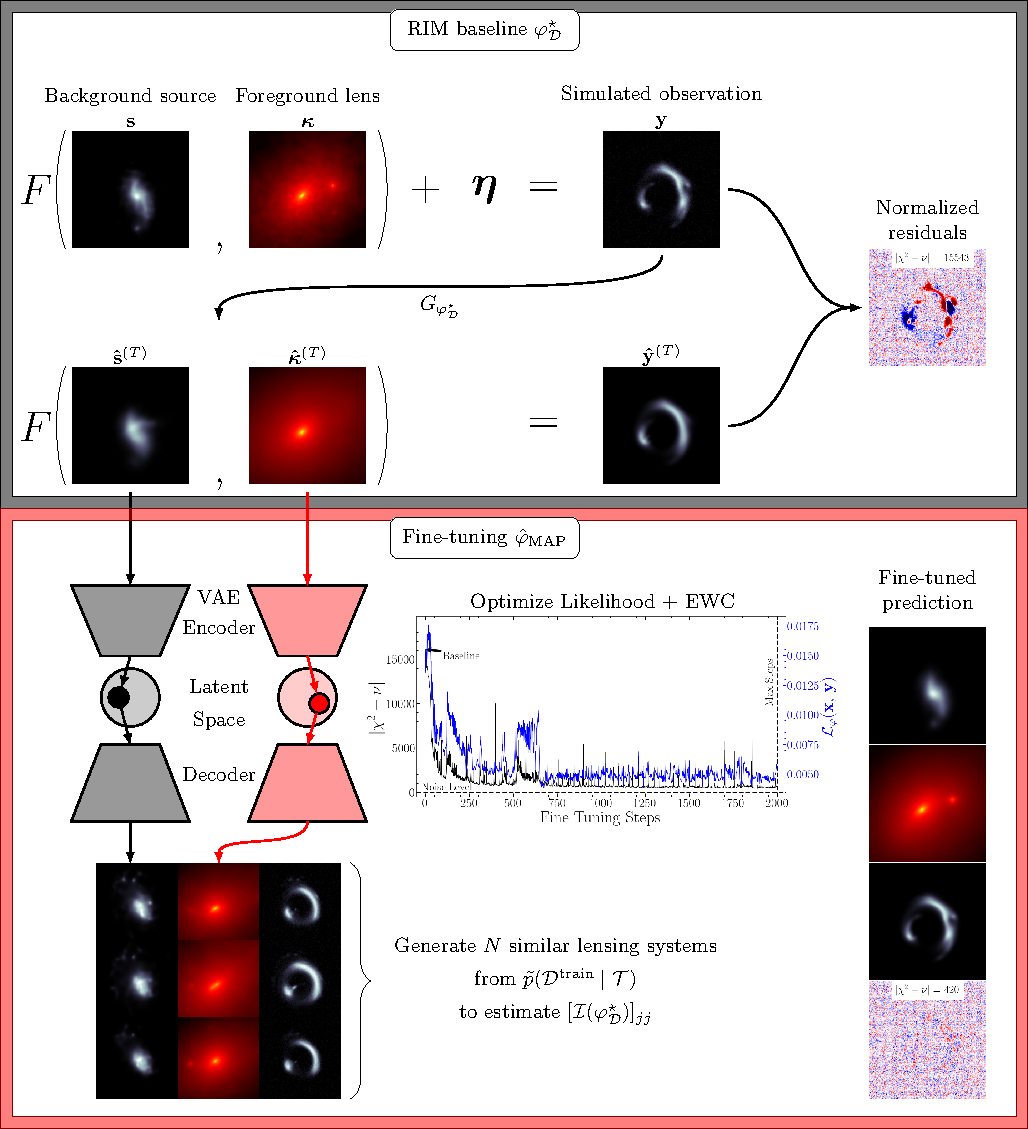
\includegraphics[width=0.9\textwidth]{figures/main_figure}
        \caption{A summary of the main concepts explored in this paper. First, 
        a source and convergence map are used to produce a noisy observation. This observation 
        is the input of the RIM baseline model $G_{\varphi_{\mathcal{D}}^{\star}}$, which 
        recovers the source and convergence map. The observed data is compared with 
        the RIM prediction using normalized residual maps. To achieve noise level reconstruction 
        ($\chi^2_\nu \simeq 1$), 
        the model is fine-tuned by a likelihood optimization regularized by Elastic Weight Consolidation (EWC). 
        We show the steps 
        to generate a dataset from the conditional $\tilde{p}(\mathcal{D}^{\mathrm{train}} \mid \mathcal{T})$ 
        using two VAE and the baseline prediction. 
        These samples are used to compute the diagonal elements of the 
        Fisher matrix $[\mathcal{I}(\varphi_{\mathcal{D}}^{\star})]_{jj}$.
}
        \label{fig:main figure}
\end{figure*}


A RIM \citep{Putzky2017} is a form of learned gradient-based inference
where the gradient of the likelihood is projected 
by a gradient model $g_\varphi$ 
such that
\begin{equation}\label{eq:RIM} 
\begin{aligned}
        \mathbf{\hat{x}}^{(t)} &= \mathbf{\hat{x}}^{(t-1)} 
        + g_\varphi \big(\mathbf{\hat{x}}^{(t-1)},\, \mathbf{y},\, \grad_{\mathbf{y} \mid \mathbf{\hat{x}^{(t-1)}}}\big);\\[2pt]
        t &\in \{1,\,\dots,\,T\}.
\end{aligned}
\end{equation}
We used \citet{Putzky2017}'s notation to refer to the gradient of the likelihood (${\grad_{\mathbf{y} \mid \mathbf{x}} \equiv 
\grad_{\mathbf{x}} \log p(\mathbf{y} \mid \mathbf{x})}$).
The parameters of the gradient model are shared across time ($t$). This 
choice reduces the computational complexity of optimizing $\varphi$. 
It also assumes that the governing rule of sequence \eqref{eq:RIM} should be independent of time.
The architecture of the gradient model is described in section 
\ref{sec:gradient model}.

In an earlier work related to the RIM by \citet{Andrychowicz2016}, 
equation \eqref{eq:RIM} was introduced as a form 
of optimization based meta-learning. 
The gradient model would only take as input the 
gradient of an objective function relative to another network's parameters. 
In the work of 
\citet{Putzky2017}, it was observed that \eqref{eq:RIM} could be generalized to any 
kind of inference problems by adding as input 
the estimated solution $\mathbf{\hat{x}}^{(t)}$ to the gradient model. They interpreted 
this as giving the model an awareness of its absolute position in $\mathcal{X}$. It is also 
consistent with the idea of merging the prior in the implicit structure of the 
model parameters $\varphi$. In this work, we observe that inputting the observed datum 
$\mathbf{y}$ in the gradient model adds flexibility to the inference by learning the 
initialization of the parameters as well. 

Initialization can be performed by selecting a constant value 
\citep[e.g.][]{Morningstar2018,Morningstar2019}
or by using an approximate inverse of the forward model ($\hat{F}^{-1}$) 
to estimate 
$\mathbf{\hat{x}}_0$ from the observed data \citep[e.g.][]{Lonning2019}. 
With our approach, 
the initialization takes the form
\begin{equation}\label{eq:Initialisation} 
        \mathbf{\hat{x}}^{(0)} = g_\varphi(0, \mathbf{y}, 0).
\end{equation} 
This is a \textit{learned} approximate inverse to the forward model. We note that 
merging the inverse $\hat{F}^{-1}$ inside the gradient model is not strictly necessary. 
A separate architecture could be learned before or during the 
optimisation of the gradient model. Such a design choice might be preferable 
in the case where the dimensionality of the observation and the parameters 
differs substantially.

Crucially, this adds an inductive 
bias that makes our MAP optimization problem more manageable. 
The learned initialization
will favour an explicit mapping between 
$\mathcal{Y}$ and the region of $\mathcal{X}$ with a high prior 
probability density --- that is, the region of 
the parameter space where the training dataset labels are found.
Without this, information about the observation
would only be filtered through the gradient of the likelihood. 
Since the likelihood is not a globally convex function, 
a first order method like the RIM will often fail to converge to 
the MAP if the starting solution $\hat{\mathbf{x}}^{(0)}$ 
is far from the MAP. The gradient of the likelihood, in that situation, 
would point toward a local minima that will conflict 
with the loss function $\mathcal{L}_\varphi$ minima, thus making the optimisation 
of the gradient model more difficult.
If we suppose that an approximate inverse $\hat{F}^{-1}(\mathbf{y})$ exists
--- given a dataset $\mathcal{D}$ ---
and bake this function into the neural net architecture, then the RIM
can take full advantage of the gradient information in the neighborhood of the 
MAP in $\mathcal{X}$.

%We 
%conjecture that the architecture of the gradient model 
%(described in section \ref{sec:gradient model}) can 
%make better use of the information contained in the observed 
%vector $\mathbf{y}$ than it can using the 
%gradient of the likelihood alone $\grad_{\mathbf{y} \mid \mathbf{x}}$
%in regards of the first step of the recurrence.

\begin{figure}
        \centering
        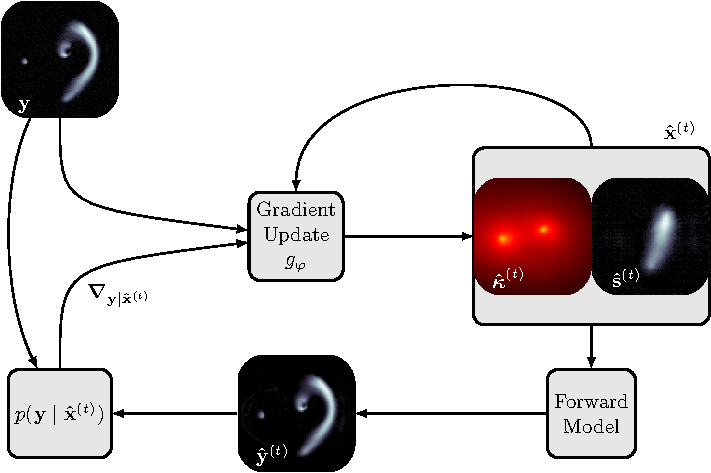
\includegraphics[width=\linewidth]{figures/schematic_rim}
        \caption{Rolled computational graph of the RIM.}
        \label{fig:rolled_graph}
\end{figure}

\begin{figure*}[ht!]
        \centering
        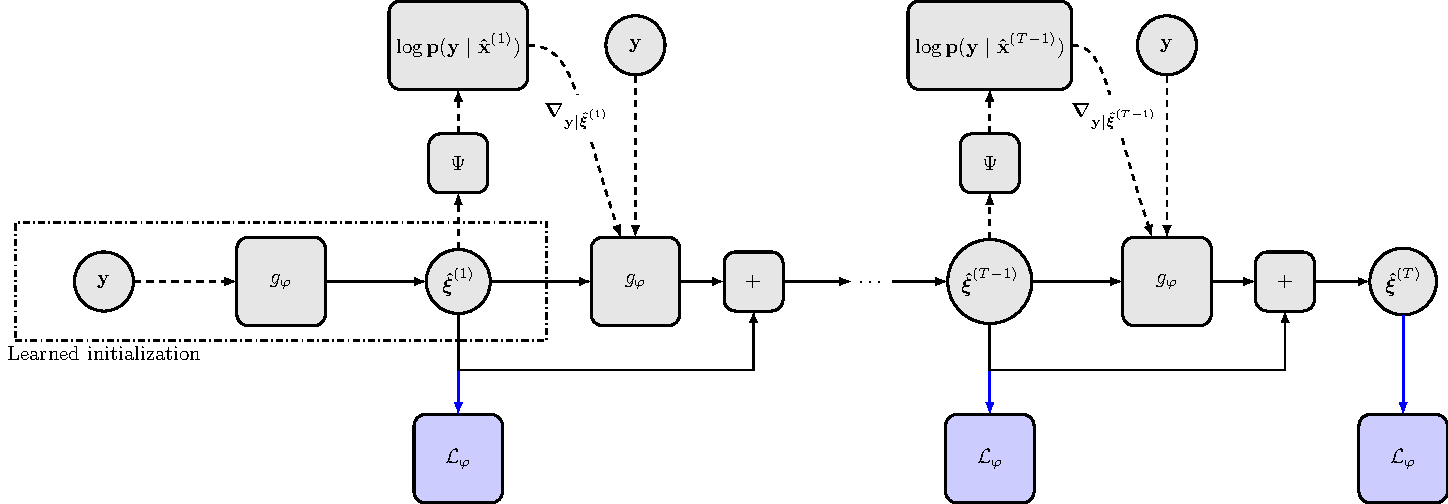
\includegraphics[width=\linewidth]{figures/schematic_rim_unrolled}
        \caption{Unrolled computational graph of the RIM. Operations along solid arrows are being 
        recorded for BPTT, while operations along dashed arrows are not. The blue arrows are only 
        used for optimisation during training. During fine-tuning or testing, the loss is computed only 
        as an oracle metric to validate that our methods can recover the ground truth.}
        \label{fig:unrolled_graph}
\end{figure*}

\begin{figure*}[ht!]
        \centering
        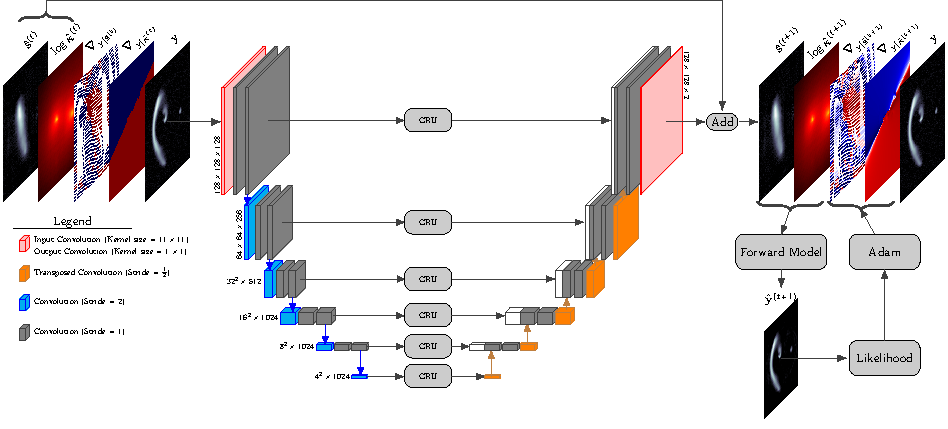
\includegraphics[width=\textwidth]{figures/unet_architecture.pdf}
        \caption{
A single time step of the unrolled computation graph of the RIM.
GRU units are placed in the skip connections to guide the 
reconstruction of the source and convergence. A schematic of the steps to compute 
the likelihood gradients is shown in the bottom right of the figure, including the 
Adam processing step. The $\oplus$ symbol refer to an addition operation. See
the recurrent relation \ref{eq:RIM}.
}
        \label{fig:unet}
\end{figure*}

When optimizing the gradient model on the training dataset, 
we use a standard recurrent neural net (RNN) objective
where the loss at each step is accumulated and gradients 
are backpropagated through time (BPTT). 
The loss for each individual step is a weighted mean squared error 
over the M pixels of the labels, such that the total loss is
\begin{equation}\label{eq:Loss}
        \mathcal{L}_\varphi(\mathbf{x}, \mathbf{y}) = 
        \frac{1}{T}\sum_{t=1}^{T}\sum_{i=1}^{M} \mathbf{w}_i ([G_\varphi(\mathbf{y})]^{(t)}_i - \mathbf{x}_i)^2.
\end{equation} 
We use the notation $[G_\varphi(\mathbf{y})]^{(t)}_i$ to refer to $i^{\text{th}}$ pixel of 
the RIM prediction 
at step $t$ of the recurrent relation \eqref{eq:RIM}. When omitted, 
we assume $G_\varphi(\mathbf{y}) = [G_\varphi(\mathbf{y})]^{(T)}$.
Throughout this 
paper, we will make a distinction 
between the loss function $\mathcal{L}_\varphi$
and the cost (also called empirical risk), 
which is defined as the 
expectation of the loss over a dataset $\mathcal{D}$.
The RNN optimisation problem is to minimize the cost:
\begin{equation}\label{eq:Cost} 
        \hat{\varphi} = \underset{\varphi}{\text{argmin}}\,\,
        \mathbb{E}_{(\mathbf{x},\mathbf{y}) \sim \mathcal{D}}\big[
        \mathcal{L}_\varphi(\mathbf{x}, \mathbf{y}) \big].
\end{equation} 

We follow previous work in setting a uniform weight over the time 
steps ($\mathbf{w}^{(t)} = \frac{\mathbf{w}}{T}$). 
The choice of the pixel weights $\mathbf{w}_i$ is informed 
by our physical intuition about the problem. This specific choice is discussed 
in section \ref{sec:baseline training}.

In figure \ref{fig:unrolled_graph}, we show the unrolled computational graph of the RIM. 
During training of the gradient model $g_\varphi$, operations along the solid arrows are being 
recorded for BPTT. The recording is stopped along the dashed arrow since these operations 
are part of the forward modelling process.
By avoiding the computation of these gradients, training time is reduced and 
knowledge about the inner workings  
of a specific likelihood (and forward model) is insulated from the optimization algorithm.
This is analogous to a common RNN use-case like text generation, where the process responsible 
for producing the next element in a time series is a black box to the optimization 
algorithm. 

The gradient of the likelihood is computed using automatic differentiation. Following 
\citep{Modi2021}, we preprocess the gradients using the Adam algorithm \citep{Kingma2013}. 
For clarity, we only illustrated this step in Figure \ref{fig:unet}. 


\subsection{The Gradient Model}\label{sec:gradient model}


The neural network architecture is illustrated in Figure \ref{fig:unet}, which shows 
a single time step of the unrolled computation graph of the RIM.
We use a U-net \citep{Ronneberger2015} architecture 
with Gated Recurrent Units \citep[GRU:][]{Cho2014} placed in each skip connections. 

Each GRU cell has it's own memory tensor that is updated through time at each iteration of 
equation \ref{eq:RIM}. The shape of a memory tensor is set to match the
feature tensor fed into it from the parent layer in the network graph. 
Instead of learning a compressed representation like in the hourglass
architecture (i.e. autoencoder), the U-net architecture naturally separates the spatial 
frequency components of the signal into its vertical levels. The first level generally encodes 
high frequency features while the lower level encodes low frequency features (due to downsampling of the feature maps). 
Adding an independent memory unit 
at each level preserve this property.

Convolutional layers with a stride of 2 are used for downsampling, while 
stride of $\frac{1}{2}$ are used for upsampling of the feature maps 
(identified in blue and orange respectively in figure \ref{fig:unet}). 
Most layer use a kernel size of $3\times3$, except the first and last layer. 
The first layer has 
larger receptive field ($11\times11$) to capture more details in the input tensor, 
while the last layer has kernels of size $1\times 1$. 
A $\tanh$ 
activation function is used 
for each convolutional layer, including strided convolutions, except for the output 
layer. 
% We found that this choice is generally better than other popular activation functions like
% the leaky ReLU. 
%We conjecture that the symmetry of $\tanh$ around 0 encodes the task 
%of computing a gradient better than its counterparts. 
%Another possible 
%explanationi

The U-net outputs an image tensor with two channels, one dedicated for the update of the source 
and the other to the update of the convergence (see figure \ref{fig:unet}). 

Finally, we must address the notion of preprocessing in the context of a RIM. Since the 
prediction of the neural network are processed by a forward model during the inference, 
preprocessing must be implemented as a part of the RIM architecture. We use the notion 
of link function $\Psi: \Xi \rightarrow \mathcal{X}$ 
introduced by \citet{Putzky2017}, which is defined as an invertible transformation 
between the network prediction space $\boldsymbol{\xi} \in \Xi$ 
and the forward modelling space $\mathcal{X}$. The 
loss $\mathcal{L}_\varphi$ must be computed in the $\Xi$ space in order 
to avoid gradient vanishing problems when $\Psi$ is a non-linear mapping.
The choice for $\Psi$ is mentioned in section \ref{sec:baseline training}.


% Talk about this choice
% Shared memory is important, possibly more than the notion that source and kappa require very different 
% reconstruction procedure (because of different structure etc).

% Choice of model correspond to choosing an inductive bias, or how the function should behave 
% for points in and out of the dataset
% Generalization means the ability to make prediction about the behavior of the function 
% at novel points in the domain of the function.
% In the meta-learning framework, examples are problem instances. Generalization means to transfer 
% knowledge accross problem instances.
% The reuse of the problem structure is known as transfer learning. In the context of meta-learning, 
% this is cast as generalization.

\subsection{The Forward Model}\label{sec:forward model}

An observation is simulated by ray tracing the brightness distribution 
of the background source to the foreground coordinate system. 
In our case, the coordinate systems have discretized representations.
Each pixel of an image is labeled with a subscript index $i$, which 
we distinguish from a parenthesized superscript index $(i)$ that refers to 
the member of a set or list of tensors. For clarity, we omit 
the superscript index in what follows.

Each pixel is associated 
with an intensity value and a coordinate vector.
The foreground pixel coordinates $\boldsymbol{\theta}_i$ and the source 
pixel coordinates $\boldsymbol{\beta}_i$ are related by
the lens equation
\begin{equation}\label{eq:LensEquation}
        \bm{\beta}_i = \bm{\theta}_i - \bm{\alpha}(\bm{\theta}_i),
\end{equation}
where $\boldsymbol{\alpha}$ is a deflection angle.
It is obtained from the projected surface 
density field $\kappa$ --- also referred to as convergence --- by the integral
\begin{equation}\label{eq:alpha}
        \bm{\alpha}(\boldsymbol{\theta}_i) = 
        \frac{1}{\pi} \int_{\mathbb{R}^2}
        \kappa(\boldsymbol{\theta}') 
        %\underbrace{
        \frac{\boldsymbol{\theta}_i
        - \boldsymbol{\theta}'}{\lVert \boldsymbol{\theta}_i - 
        \boldsymbol{\theta}' \rVert^2}
%}_{\displaystyle \boldsymbol{\omega}(\boldsymbol{\theta_i} -\boldsymbol{\theta'})} 
        d^2\boldsymbol{\theta}'
\end{equation}
The intensity of a pixel in a simulated observation
is obtained by bilinear interpolation of the 
source brightness distribution at the coordinate $\boldsymbol{\beta}_i$.
In this work, the convergence also has a discrete representation. Thus, 
we approximate this integral by a discrete global convolution. Taking 
advantage of the convolution theorem, this operation 
can be computed in near-linear time using 
the Fast Fourier Transform (FFT). 

Assuming the observation 
has $M^2$ pixels, the convolution kernel %$\boldsymbol{\omega}$ 
would have $(2M + 1)^{2}$ pixels. 
Both the convergence tensor and the kernel tensor are zero-padded 
to a size of $(4M+1)^{2}$ pixels in order to approximate a linear 
convolution and significantly reduce aliasing.

A blurring operator --- convolution by a point spread function --- is then 
applied to the lensed image to replicate the response of an imaging system. 
This operator is implemented as a GPU-accelerated matrix operation 
since the blurring kernels used in this paper have a significant proportion
of their energy distribution encircled inside a small pixel radius. 

\subsection{Fine-Tuning}\label{sec:fine-tuning}

\subsubsection{Objective function}
Once the gradient model is trained, the RIM is a baseline 
estimator of the parameters $\mathbf{x}$ given a noisy observation $\mathbf{y}$. 
We now concern ourselves with a strategy to improve 
this estimator without having to retrain the gradient model from scratch. 
This is important 
for high SNR observation, where attaining noise level reconstruction 
gets exponentially more difficult.

The metric for the goodness of fit 
is the reduced chi squared $\chi^2_\nu = \frac{\chi^2}{\nu}$.
$\nu$ is the total number of degrees of freedom. 
In this work, $\nu$ is the amount of pixels in $\mathbf{y}$.
Generally, our goal will be to reach $\chi^2_\nu = 1$, where 
the residuals have reached noise level. We will 
also use the chi squared difference $|\chi^2 - \nu|$ when 
the reduced chi squared is very close to 
1 to distinguish between reconstructions that reach noise 
level and those that still need improvement.

The $\chi^2$ metric by itself is not sufficient to judge the quality 
of a reconstruction. This is why the full residual maps 
will be provided in the result section as well. 

The fine-tuning objective is to minimize directly the $\chi^2$:
\begin{equation}\label{eq:MAP} 
        \hat{\varphi}_{\mathrm{MAP}} = \underset{\varphi}{\mathrm{argmax}}\,\, 
        \frac{1}{T}\sum_{t=1}^{T} \log p(\mathbf{y} \mid [G_\varphi(\mathbf{y})]^{(t)}) + \log p(\varphi).
\end{equation} 
Unlike the squared loss \eqref{eq:Loss}, this objective function is implicit 
and makes no use of labels. 
%(${p(\mathbf{y} \mid \mathbf{x}): \mathcal{Y} \times \mathcal{Y} \rightarrow \mathbb{R}}$, 
%see equation \eqref{eq:Likelihood}).
This allows us to use this objective at test time. 

\subsubsection{Transfer Learning}
We now address the issue of transferring knowledge from a training task 
(problem \eqref{eq:Cost}) to a specific test task (problem \eqref{eq:MAP}).
The reader might refer to reviews on transfer learning \citep{Pan2010,Zhuang2019} 
for a broad overview of the field. The strategy we outline falls into 
the category of inductive transfer learning.

Since the data likelihood $p(\mathbf{y} \mid \mathbf{x})$ 
does not contain \textit{a priori} information 
about the solution $\hat{\varphi}_{\mathrm{MAP}}$,
inductive biases must be introduced to make 
the problem \eqref{eq:MAP} well-posed. 
\begin{enumerate}[label=(\subscript{\mathcal{H}}{{\arabic*}})]
        \setcounter{enumi}{3}
        \item \label{prior:initialization} Initializing $\varphi$ with a pretrained set of weights 
                that minimizes the cost over $\mathcal{D}^{\mathrm{train}}$; 
        \item \label{prior:early stopping} Early stopping when a maximum number of steps is reached or 
                $\chi^2_\nu \leq 1$;
        \item \label{prior:learning rate} Using a small learning rate.
\end{enumerate}
\ref{prior:early stopping} and \ref{prior:learning rate} encode the assumption 
that the optimal estimator is to be found \textit{near} the initialization.

As it turns out, \ref{prior:initialization} is not strong 
enough to preserve the knowledge learned during pretraining. 
This has long been observed in the literature and was coined as the 
catastrophic interference phenomenon in 
connectionist networks \citep{McCloskey1989,Ratcliff1990}.
In summary, a sequential learning problem exhibits catastrophic 
forgetting of old knowledge when confronted with new examples (possibly 
from a different distribution or process), in a manner 
\begin{enumerate}[label=(\subscript{\mathrm{CF}}{{\arabic*}})]
        \item \label{cf:steps} proportional to the amount of learning;
        \item \label{cf:weights} strongly dependant to the disruption of the parameters
                involved in representing the old knowledge.
\end{enumerate}
While \ref{prior:early stopping} and \ref{prior:learning rate} can 
potentially alleviate \ref{cf:steps}, \ref{cf:weights} is not 
trivially addressed by the inductive biases introduced so far.

We follow the work of \citet{Kirkpatrick2016} to define a prior distribution
over $\varphi$ that address this issue.
We denote the pretrained weights with $\varphi_{\mathcal{D}}^{\star}$ 
and the Fisher information matrix with $\mathcal{I}$:
\begin{equation}\label{eq:Prior} 
        \log p(\varphi) = -\frac{\lambda}{2}\sum_{j} [\mathcal{I}(\varphi_{\mathcal{D}}^{\star})]_{jj} 
        (\varphi_j - \varphi_{\mathcal{D},j}^{\star})^{2}.
\end{equation} 
We've included a derivation 
of this term in the appendix \ref{ap:ewc}. 
The elements of the Fisher 
matrix are computed using examples from the training 
dataset that are similar to the observed lensing system 
$\mathbf{y}$. 

%By definition, the Fisher matrix is the 
%expected value of the observed information that 
%the examples carry about $\varphi$. 

%Another way to view this term is by noting that 
%the inverse of the Fisher diagonal is the Cramér-Rao \citep{Rao1945,Cramer1946} 
%lower bound estimate of the variance 
%of the network parameters. A large variance 
%implies $\varphi_i$ carries little 
% information about the examples.

%It's probably easier to understand this term just in term of the score. 
%How much does the likelihood varies w.r.t to the network parameters?
% The more the likelihood, the more information the parameters carry.

We use the notation $\mathcal{T}$ to 
symbolize the random variable related to the event 
of observing an image $\mathbf{y}$, a noise covariance $C$ 
and a PSF $\Pi$ such that $(\mathbf{y},\,C,\,\Pi) \sim \mathcal{T}$.
Thus, the distribution of elements 
from the training dataset $\mathcal{D}^{\mathrm{train}}$ 
that are similar to task $\mathcal{T}$ can be 
modeled by the conditional distribution 
$p(\mathcal{D}^{\mathrm{train}} \mid \mathcal{T})$.

This distribution is intractable in general. Instead, we 
use the VAE trained on the training dataset labels as a surrogate 
distribution of the prior $\tilde{p}(\mathbf{x})$.  
After having observed $\mathcal{T}$, we can fully define 
the \textit{noisy} forward model (equation \eqref{eq:MainEquation}) 
using $C$ and $\Pi$ which gives us a surrogate of 
the conditional 
${(\tilde{\mathbf{x}}^{(i)},\, F(\tilde{\mathbf{x}}^{i}) + \boldsymbol{\eta}) \sim \tilde{p}(\mathcal{D}^{\mathrm{train}} \mid C,\, \Pi)}$.
The point estimate $\mathbf{\hat{x}}^{(T)}$ of the baseline RIM 
is used in conjonction with the encoder network of the VAE to 
constrain our sampling of the latent space 
to the region centered around the predicted mean of the latent code. 
This step 
conditions the surrogate prior on $\mathbf{y}$.
These ideas are 
illustrated in figure \ref{fig:main figure}. 


%We can, however, make use of theoretical and 
%experimental evidence that overparametrized 
%neural networks exhibits a spectral bias \citep{Rahman2018} 
%toward learning low frequencies first during training. We observe 
%that the baseline model generally 
%provides a coherent prediction ($\gamma(k) = 1$) in the low frequency 
%regime, which is consistent with a spectral bias hypothesis. 
%This suggest a possible approach to ground our method. 
%The MLE-optimal estimator should at least 
%preserve the low frequency features predicted by the baseline. 
%Otherwise, we might suspect that the optimisation procedure 
%has found a degenerate solution that is not consistent with the 
%prior learned by the baseline.

%This also points to interesting strategies that could alleviate 
%overfitting. For instance, freezing the deeper layers of the U-net during 
%fine-tuning might preserve the low frequency features learned during pretraining. 
%This is also suggested as a strong regularization method in \citet{Li2018}. 
%We explore such ideas in the appendice


\section{Data}\label{sec:data}



\subsection{COSMOS}\label{sec:source}
Our sources brightness distributions are taken from the Hubble Space Telescope (HST) 
Advanced Camera for Surveys Wide Field Channel COSMOS field \citep{Koekemoer2007,Scoville2007},
a $1.64\,\mathrm{deg}^{2}$ contiguous survey acquired in the F814W filter. 
A dataset of mag limited ($\mathrm{F814W} < 23.5$) deblended galaxy postage stamps \citep{Leauthaud2007} was compiled as 
part of the GREAT3 challenge \citep{Mandelbaum2014}. The data is 
publicly available \citep{Mandelbaum2012}, and the preprocessing is done through the open source software 
\texttt{GALSIM} \citep{Rowe2015}. \par
\begin{figure}
        \centering
        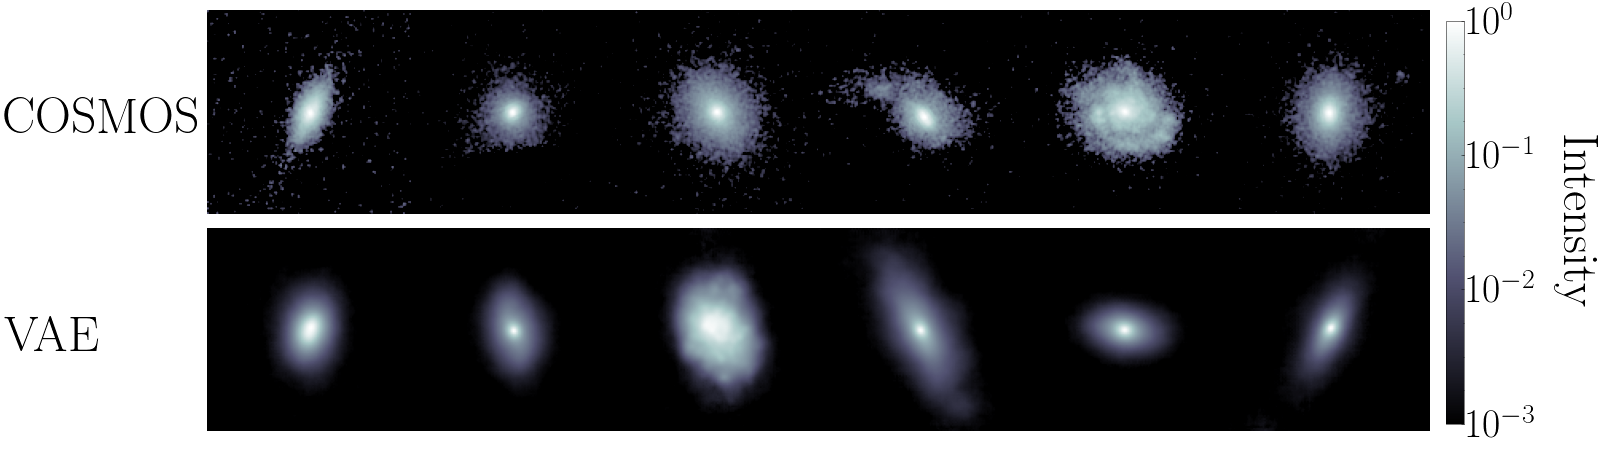
\includegraphics[width=\linewidth]{figures/gal_vae_sample}
        \caption{Examples of COSMOS galaxy images 
                (top row) and VAE generated samples (bottom row) used as labels in $\mathcal{D}^{\mathrm{train}}$.}
        \label{fig:source}
\end{figure}
We applied the 
\texttt{marginal} selection criteria (see the \texttt{COSMOSCatalog} class) and imposed a flux per image
greater than $50\,\,\mathrm{photons}\,\,\mathrm{cm}^{-2}\,\mathrm{s}^{-1}$. 
This final set has a total of 13\,321 individual images.
Each image is convolved with its original PSF and drawn into a postage stamps of $158^2$ pixels. 
They are then 
background subtracted, randomly shifted and rotated by an angle of $90^\circ$. They are finally 
cropped to a $128^2$ image. 
Random augmentations are applied only once per image, leaving the size of the dataset unchanged.
The small amount of noise that is left in each image is removed using an autoencoder. 
Details regarding this 
procedure are found in the appendix \ref{ap:AE}. 
Finally, pixel intensity is 
normalized in the range $[0,1]$.

The final augmented set is then split into a training set (90\%) and a test set (10\%). 
The training set is used to train a VAE and produce simulated observations 
to train the RIM.


\subsection{IllustrisTNG}\label{sec:kappa}
\subsubsection{Smooth Particle Lensing}\label{sec:SPL}
To compute a convergence map from an N-body simulation, 
we follow \citet{Auger2007} in treating 
each particle as flow tracers instead of describing their density as Dirac $\delta(\mathbf{r})$. Smoothing 
each particle density on a non-singular kernel reduces the particle noise affecting all 
important lensing quantities --- most importantly the convergence. At the same time, the choice of the kernel size 
is important to preserve substructures in the 
lens that we might potentially be interested in. Following \citet{Rau2013}, we use Gaussian 
smoothing with an adaptive kernel size determined by the distance of the 64\textsuperscript{th} nearest neighbours of 
a given particle $D_{64,i}$. 
\begin{equation}\label{eq:Ksmooth}
\begin{aligned}
    \kappa(\mathbf{x}) &= \frac{1}{\Sigma_{\mathrm{crit}}} \sum_{i=1}^{N_{\mathrm{part}}}
        \frac{m_i}{2 \pi \hat{\ell}^2_i} 
        \exp \left(-\frac{1}{2} \frac{(\mathbf{x} - \mathbf{x}_i)^2}{\hat{\ell}_i^2}  \right) \\
    \hat{\ell}_i &= \sqrt{\frac{103}{1024}}D_{64,i}.
\end{aligned}
\end{equation}
The nearest neighbours are found by fitting a k-d tree ---  implemented in 
\texttt{scikit-learn} \citep{scikit-learn} --- 
to the $N_{\mathrm{part}}$  particles 
in a cylinder centered on the centre of mass of the halo of interest.
We canonically defined the critical surface density
\begin{equation}\label{eq:Scrit}
\Sigma_{\mathrm{crit}} = \frac{4 \pi G}{c^ 2} \frac{D_\ell D_{\ell s}}{D_s}.
\end{equation}
$D_\ell$, $D_s$ and $D_{\ell s}$ are angular diameter distance to the lens, source and between the lens and the source respectively, 
$G$ is the gravitational constant and $c$ the speed of light.

\subsubsection{Data augmentation}
We used the last snapshot (redshift $z=0$) 
of the IllustrisTNG-100 simulation \citep{Nelson2018} to get 
physically plausible realizations of dark matter and baryonic matter halos.
For our purposes, dark matter halos are synonymous with \texttt{subhaloes} in the data and 
galaxy clusters are associated with \texttt{halos}. %\citep()

\begin{figure}
        \centering
        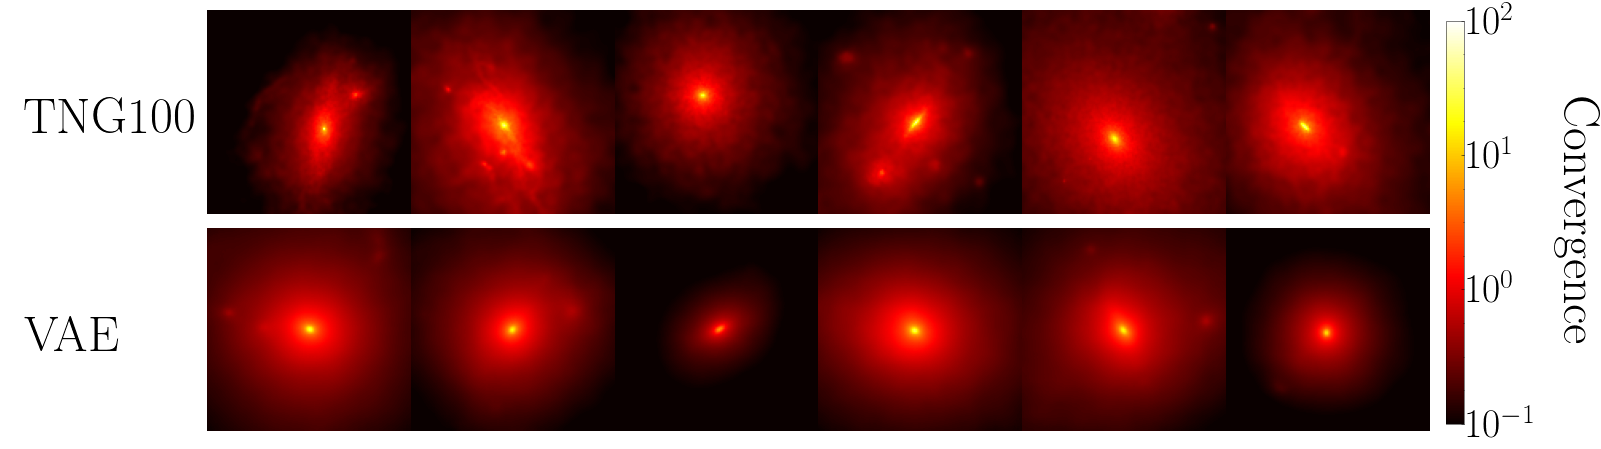
\includegraphics[width=\linewidth]{figures/kap_vae_sample}
        \caption{Examples of smoothed Illustris TNG100 convergence map (top row) 
        and VAE generated samples (bottom row) used as labels in $\mathcal{D}^{\mathrm{train}}$.}
        \label{fig:kappa}
\end{figure}

We select 1604 halos with the criteria that they have a total
dark matter mass of at least $9\times10^{11} M_{\odot}$. We then collect all 
dark matter, gas, stars and black holes particles from the data associated to the galaxy 
cluster within which the halo resides in to create a smoothed projected surface density maps 
around the centroid of the halo as prescribed in section \ref{sec:SPL}.

We adopt the $\Lambda$CDM cosmology from 
\citet{PlanckCollaboration2018} with $h=0.68$ to compute 
angular diameter distances. We also fix the 
source redshift to $z_s=1.5$ and the deflector redshift to $z_\ell=0.5$. 
We note that changing the redshifts or the cosmology 
only amount in a rescaling of the $\kappa$ map by a global scalar.
The smoothed distributions from equation \eqref{eq:Ksmooth} are 
rendered into a regular grid of $188^2$ pixels with a comoving field of view of $105\,\,\mathrm{kpc}/h$. 
To avoid 
edge effects in the pixelated maps, we include particles outside of the field of view in the sum of equation \eqref{eq:Ksmooth}.
\par
Before applying augmentation or considering different projections, our dataset of halos is split into a 
training set (90\%) and a test set (10\%).
We take 3 different projections ($xy$, $xz$ and $yz$) of the 3D particle 
distribution, which amount to a total of $4\,812$ individual maps. 
Random $90^{\circ}$ rotations and random shift to the pixel coordinates are applied to each 
image. The $\kappa$ maps are then rescaled by a random factor to change their 
estimated Einstein radius to the range 
$[0.5,\,2.5]$ arcsec.
The Einstein radius is defined as
\begin{equation}\label{eq:ThetaE}
        \theta_E = \sqrt{\frac{4GM(\theta_E)}{c^ 2} \frac{D_{\ell s}}{D_\ell D_s}}
\end{equation} 
where $M(\theta_E)$ is the mass enclosed inside the Einstein radius. In practice, we estimate this quantity 
by summing over the mass of pixels with a value greater than the critical density ($\kappa > 1$). 
For data augmentation purposes, this rough definition gives a good enough estimate of the 
size of the lensed image that will be produced by some $\kappa$ map, 
circumventing the fact that the Einstein radius does not have a proper definition for most of the convergence fields of 
hydrodynamical simulations.
We test multiple scaling factors for each $\kappa$ map, then uniformly sample between those that produce an estimated 
Einstein radius within the 
desired range. This step is used to remove any bias in the Einstein radius that might come from the mass function 
of the simulation. 

The final maps are cropped down to $128^2$ pixels.
Placed at a redshift $z_\ell=0.5$, a $\kappa$ map will thus span an angular field of view of $7.69''$ with 
a resolution similar to HST. This field of view is wide enough to cover a typical gravitational 
lens observed in the sky, which partly justify our choice for the comoving field of view earlier. 

With these augmentation procedures, a total of $50\,000$ maps are created from the training split and 
$5\,000$ from the test split.
The training set is used to train a VAE and produce simulated observations 
to train the RIM. 
\begin{figure*}[ht!]
        \centering
        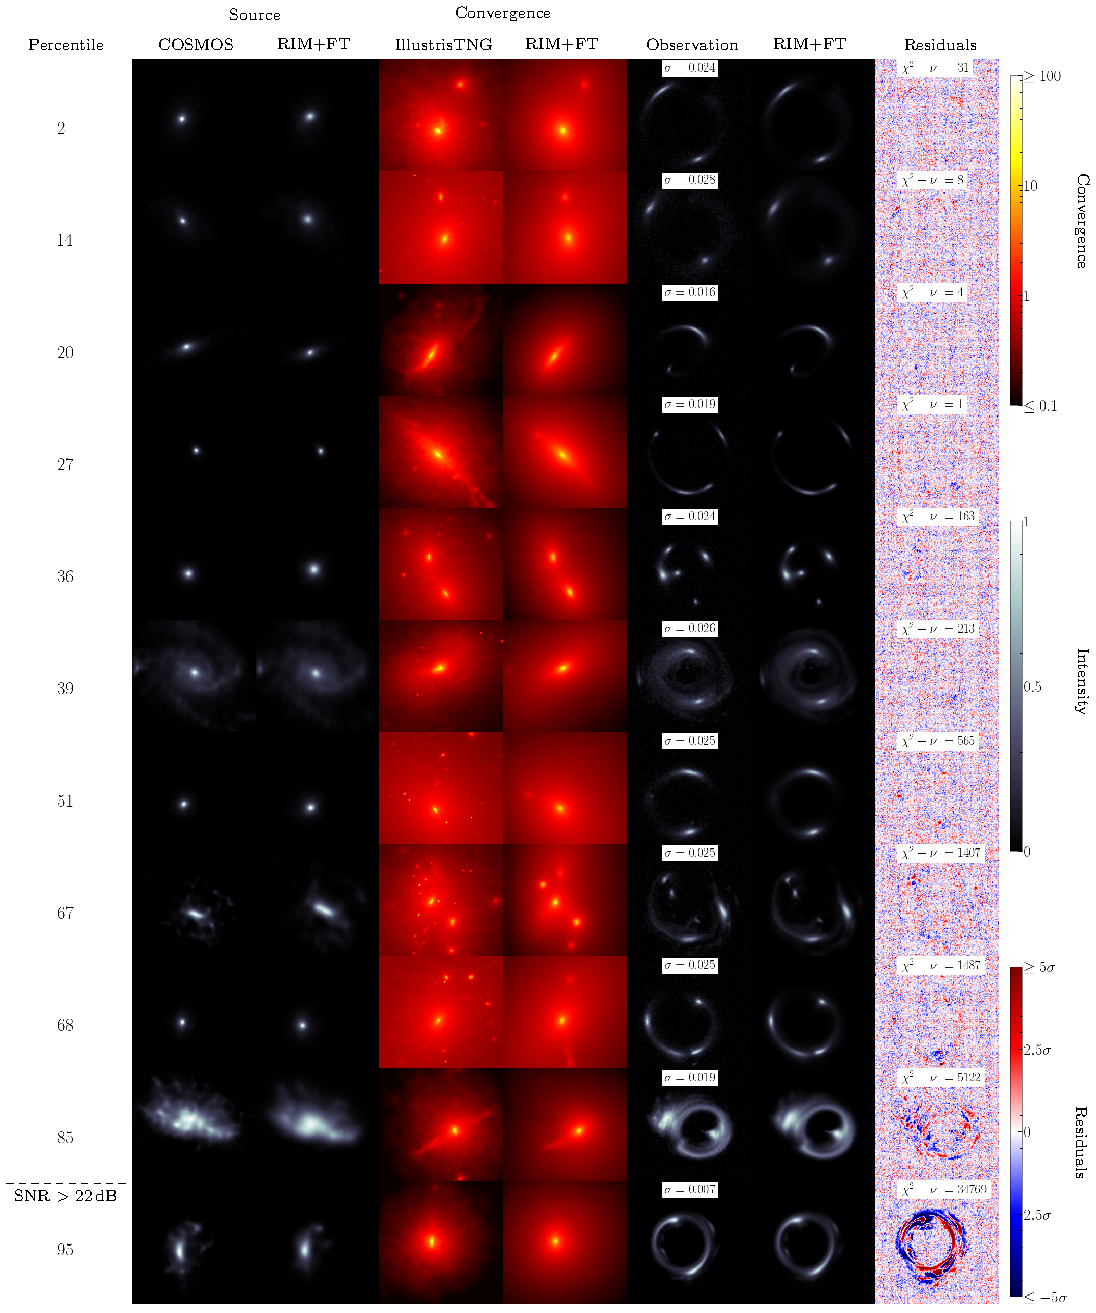
\includegraphics[width=0.9\textwidth]{figures/main_result}
        \caption{
                Cherry-picked sample of the fine-tuned RIM reconstructions 
                on a test set of 3000 examples. 
                Examples are ordered from the best $\chi^2$ (top) to the worst (bottom). 
                The percentile rank of each example is in the leftmost column. 
                The last example 
        shown has SNR above the threshold defined in Figure \ref{fig:chi squared vs noise}.
} 
        \label{fig:main result}

        \newpage
\end{figure*}

\subsection{Simulated Observations}\label{sec:simulated observation}
Having defined a source map and a convergence map, we apply the ray tracing simulation 
prescribed in section \ref{sec:forward model} to produce an observation 
with observational effects that roughly corresponds to HST images. 

For each observation, a Gaussian point spread function is 
created with a full width at half maximum (FWHM) 
randomly generated from a truncated normal distribution.
The support of the distribution is truncated below by the 
angular size of a single pixel and above by the angular size of 4 pixels. 
White noise with a standard deviation randomly generated from a truncated normal distribution 
is then added to the convolved observation to simulate SNR conditions between 
$10\,\mathrm{dB}$ and $30\,\mathrm{dB}$. For simplicity, we define $\mathrm{SNR} = \frac{1}{\sigma}$. 
This definition is equivalent to the peak signal-to-noise ratio. 

We set the observed image field of view to match with the convergence field view ($7.69''$). 
We choose the background field of view to be $3''$.
As a validation criteria for each simulated image, we impose 
a minimum magnification of 3. Thus, 
we make sure that most pixel coordinates in the image plane will be mapped inside the 
source coordinate system through the lens equation \eqref{eq:LensEquation}. 

\begin{table}[ht!]
\centering
\caption{Physical model parameters.}
\label{tab:phys}
\begin{tabular}{ccc}
        Parameter &  Distribution/Value \\
        \hline \hline
        Lens redshift $z_\ell$ & $0.5$ \\
        Source redshift $z_s$ & $1.5$ \\
        Field of view ('') & $7.69$ \\
        Source field of view ('') & $3$ \\
        PSF FWHM ('') & $\mathcal{TN}(0.06,\, 0.3;\, 0.08,\, 0.05)$
        \footnote{We defined the parameters of the truncated normal in the order $\mathcal{TN}(a,\, b;\, \mu,\, \sigma)$, where $[a,\, b]$ defines the support of the distribution.} \\
        Noise amplitude $\sigma$ & $\mathcal{TN}(0.001,\, 0.1;\, 0.01,\,0.03)$\\
        \hline
\end{tabular}
\end{table}

$400\,000$ observations are simulated from random pairs of COSMOS sources 
and IllustrisTNG convergence training split in order to train the RIM. 
An additional $200\,000$ observations are created from pairs 
of COSMOS source and pixelated SIE convergence map are added to the dataset 
as well. The parameters for these $\kappa$ maps are listed in table \ref{tab:sie}. 

We found this addition to be beneficial to learning since it adds an 
inductive bias in the learning favoring isothermal profiles.
We expect some lensing configurations like 
large Einstein rings or double images to poorly constrain the inner structure of the 
mass distribution. Building an inference pipeline with strong constraints on the 
slope of the profile goes beyond the scope of this work. As such, imposing a prior through 
the dataset is sufficient for our goal. It is also motivated by the \textit{bulge-halo conspiracy} --- 
the observation that most lensing configurations observed in the sky can be explained 
to first order approximation by 
an average slope consistent with an isothermal profile.

\begin{table}[ht!]
\centering
\caption{SIE parameters.}
\label{tab:sie}
\begin{tabular}{ccc}
        Parameter &  Distribution \\
        \hline \hline
         Radial shift (arcsec) & $\mathcal{U}(0, 0.1)$ \\
        Azimutal shift & $\mathcal{U}(0, 2\pi)$ \\
        Orientation & $\mathcal{U}(0, \pi)$ \\
        $\theta_E$ (arcsec) & $\mathcal{U}(0.5, 2.5)$ \\
        Ellipticity & $\mathcal{U}(0, 0.6)$ \\
        \hline
\end{tabular}
\end{table}


$1\,600\,000$ simulated observations are generated from the VAE 
background sources and convergence maps as part of the training set. 
In principle, we could continuously generate examples from the VAE. 
However, having a fixed amount let us apply some validation check to each 
observation ($\mathbf{y}$) in order to avoid configuration like a
single image of the background 
source or an Einstein ring cropped by the field of view.


\section{Training}\label{sec:training}



\subsection{VAE}\label{sec:vae training}

As mentionned in \citet{Kingma2019}, direct optimisation 
of the ELBO can prove difficult because the reconstruction term $\log p_\theta (\mathbf{x} \mid \mathbf{z})$ 
is relatively weak compared to the Kullback Leibler (KL) divergence term. To alleviate this issue, 
we follow the work of \citet{Bowman2015} and \citet{Sonderby2016} in setting a warm-up 
schedule for the KL term in the ELBO (see appendix \ref{ap:VAE}), 
starting from $\beta=0.1$ up to $\beta_{\mathrm{max}}$. 

Usually, 
$\beta_{\mathrm{max}} = 1$ is considered optimal since it matches the original ELBO  
objective derived by \citet{Kingma2013}. 
But, we are more interested in the 
sharpness of our samples and accurate inference around small regions of the latent 
space for fine-tuning. Thus, setting $\beta_{\mathrm{max}} < 1$ allows us to increase 
the size of the information bottleneck (or latent space) of the VAE 
and improve the reconstruction cost of the model. 
This is a variant of the $\beta$-VAE \citep{Higgins2017}, where $\beta > 1$ was found 
to improve disentangling of the latent space \citep{Burgess2018}. 

\begin{table}[H]
        \centering
        \caption{Hyperparameters for the background source VAE.}
        \label{tab:Source VAE}
        \begin{tabular}{cc}
                Parameter & Value \\\hline\hline
                Input preprocessing & $\bbone$ \\
                                    & \\

                \textit{Architecture} & \\
                Levels (encoder and decoder) & 3 \\
                Convolutional layer per level & 2 \\
                Latent space dimension & 32\\
                Hidden Activations & Leaky ReLU \\
                Output Activation & Sigmoid \\
                Filters (first level) & 16 \\
                Filters scaling factor (per level) & 2 \\
                Number of parameters & $3\,567\,361$\\

                           & \\
                \textit{Optimization} & \\
                Optimizer & Adam \\
                Initial learning rate & $10^{-4}$ \\
                Learning rate schedule & Exponential Decay \\
                Decay rate & 0.5 \\
                Decay steps & $30\,000$ \\
                Number of steps & $500\,000$ \\
                $\beta_{\mathrm{max}}$ & 0.1 \\
                Batch size & 20\\
                \hline
        \end{tabular}
\end{table}


The value for $\beta_\mathrm{max}$ and the steepness of the schedule 
are grid searched alongside the architecture for the VAE. Our criteria 
for an optimal model is a VAE that achieve the lowest reconstruction error 
in order to produce sharp images. At the same time, the 
KL divergence should be below an empirically defined threshold to respect 
the latent space prior. 
This value is found in practice by 
manually looking at the quality of generated samples. 

For the following architectural choice, we import the notion of \textit{level} from the
U-net architecture. However, we emphasize that there is no horizontal skip connection 
in the VAE since the encoder and decoder are fundamentally separate structures and 
must be trained as such. In each level, we place a block of convolutional layers 
before downsampling (encoder) or after upsampling (decoder). These operations 
are done with strided convolutions like in the U-net architecture of the gradient 
model.

A notable element of the VAE architecture is the use of a fully connected  
layer to reshape the features of the convolutional layer into the chosen 
latent space dimension. Following the work of \citet{Lanusse2021}, we introduce 
an $\ell_{2}$ penalty between the input and output of the bottleneck 
dense layers to encourage an identity mapping. This regularisation 
term is slowly removed during training.


\begin{table}[H]
        \centering
        \caption{Hyperparameters for the convergence VAE.}
        \label{tab:Kappa VAE}
        \begin{tabular}{cc}
                Parameter & Value \\\hline\hline
                Input preprocessing & $\log_{10}$ \\
                              & \\

                \textit{Architecture} & \\
                Levels (encoder and decoder) & 4 \\
                Convolutional layer per level & 1 \\
                Latent space dimension & 16\\
                Hidden Activations & Leaky ReLU \\
                Output Activation & Linear \\
                Filters (first level) & 16 \\
                Filters scaling factor (per level) & 2 \\
                Number of parameters & $1\,980\,033$\\


                           & \\
                \textit{Optimization} & \\
                Optimizer & Adam\\
                Initial learning rate & $10^{-4}$ \\
                Learning rate schedule & Exponential Decay \\
                Decay rate & 0.7 \\
                Decay steps & $20\,000$ \\
                Number of steps & $155\,000$ \\
                $\beta_{\mathrm{max}}$ & 0.2 \\
                Batch size & 32\\
                \hline
        \end{tabular}

\end{table}



\subsection{Baseline}\label{sec:baseline training}
The choice for the pixel weight $\mathbf{w}_i$ of the loss (equation \eqref{eq:Loss})
and the link function $\Psi(\boldsymbol{\xi})$ are now addressed. 

For the source, we find that a linear link function 
(${\mathbf{\hat{s}} = \Psi(\boldsymbol{\xi}) = \bbone \boldsymbol{\xi}}$) 
is better 
than an exponential or sigmoid link function. 
Because negative pixels are not excluded, 
a ReLU is applied to the predicted source at test time. 
The weights for the source pixels are uniform.

For the convergence, we use an exponential link function with base $10$: 
$\boldsymbol{\hat{\kappa}} = \Psi(\boldsymbol{\xi}) = 10^{\boldsymbol{\xi}}$. 
This $\Psi$ encodes the non-negativity of the convergence. Furthermore, 
it is a power transformation that leaves the linked 
pixel values $\boldsymbol{\xi}_i$ normally distributed, thus improving the 
learning through the non-linearities in the neural network.

The weights of the convergence loss function are chosen to encode the fact 
that the pixel with critical mass density ($\boldsymbol{\kappa}_i > 1$) 
have a stronger effect on the lensing configuration than other pixels. 
We find in practice that the weights 
\begin{equation}\label{eq:convergence weights} 
        \mathbf{w}_i = \frac{\sqrt{\boldsymbol{\kappa}_i}}{ \sum_i \boldsymbol{\kappa}_i}, 
\end{equation} 
encode this knowledge in the loss function and improved both the empirical 
risk and the goodness of fit of the baseline model on early test runs.

The architecture of the gradient model was grid searched on 
smaller dataset ($\lesssim 10\,000$ examples) 
in order to quickly identify a small grid 
of valid hyperparameters. Then, the best hyperparameters were 
identified using a two-stage training process on the training dataset. 
In the first stage, we trained 24 different architectures from this small 
hyperparameter set for approximately 4 days (wall time using a single Nvidia A100 gpu). 
Different architectures would have a training time much longer than others, and this 
was factored in the architecture selection process. For example, adding more time 
steps ($T$) to the recurrent relation \eqref{eq:RIM} 
would yield better generalisation on the test set, but this 
would come at great costs to training time until convergence. 
Following this first stage, 4 architectures were deemed efficient enough 
to be trained for an additional 6 days. We report the hyperparameters for 
the best architecture after this second stage of training in table \ref{tab:baseline hparams}.
\begin{table}[H]
        \centering
        \caption{Hyperparameters for the baseline RIM.}
        \label{tab:baseline hparams}
        \begin{tabular}{cc}
                Parameter & Value \\\hline\hline
                Source link function & $\bbone$ \\
                $\kappa$ link function & $10^{\boldsymbol{\xi}}$ \\
                                       & \\
                \textit{Architecture} & Figure \ref{fig:unet} \\
                Recurrent steps ($T$) & 8 \\
                Number of parameters & $348\,546\,818$ \\
                                      & \\
                \textit{First Stage Optimisation} & \\
                Optimizer & Adamax \\
                Initial learning rate & $10^{-4}$\\
                Learning rate schedule & Exponential Decay \\
                Decay rate & 0.95 \\
                Decay steps & $100\,000$\\
                Number of steps & $610\,000$\\
                Batch size & 1 \\
                           & \\


                \textit{Second Stage Optimisation} & \\
                Optimizer & Adamax \\
                Initial learning rate & $6\times 10^{-5}$\\
                Learning rate schedule & Exponential Decay \\
                Decay rate & 0.9 \\
                Decay steps & $100\,000$\\
                Number of steps & $870\,000$\\
                Batch size & 1 \\
                
                \hline
        \end{tabular}
\end{table}

\begin{table}[H]
        \centering
        \caption{Hyperparameters for fine-tuning the RIM.}
        \label{tab:fine-tuning hparams}
        \begin{tabular}{cc}
                Parameter & Value \\\hline\hline
                Optimizer & RMSProp \\
                Learning rate & $10^{-6}$\\
                Maximum number of steps & $2\,000$\\
                EWC Regularizer $\lambda$ & $0.4$\\
                Number of samples from VAE & 200 \\
                \hline
        \end{tabular}
\end{table}

\section{Results}\label{sec:results}

\begin{figure*}[ht!]
        \centering
        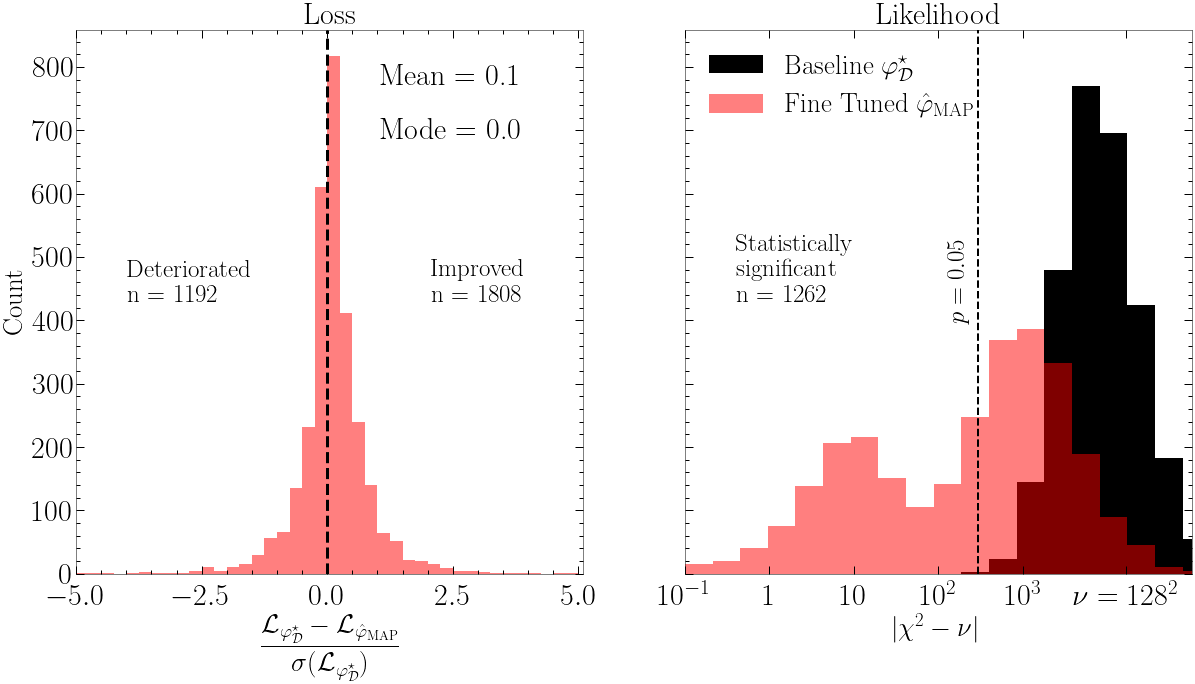
\includegraphics[width=0.8\textwidth]{figures/prior_and_likelihood}
        \caption{Summary of the goodness of fit (right panel) and loss (left panel) 
        of the fine-tuned reconstructions compared with the baseline model reconstructions 
        on the test set. The 
        $\chi^2$ is significantly improved by the optimisation. The loss, which is not directly 
        optimized during fine-tuning, is bound within $\sim 2.5\sigma$ 
        of the baseline loss because of the regularisation (EWC).
}
        \label{fig:loss and chi squared}
\end{figure*}



In this section, we present the performance of our approach 
on the held out test set. A sample of 3000 reconstruction 
problems is generated from the held-out HST and IllustrisTNG data 
with noise conditions and PSFs similar to the training set.

\subsection{Goodness of Fit}
Figure \ref{fig:main result} is a cherry picked sample of the reconstruction from the test set. 
Each reconstruction is performed by fine-tuning the baseline model 
on the observation for a maximum of 2000 steps ($\sim 20$ minutes/reconstructions on 
a single Nvidia A100 GPU). Early stopping is applied when the $\chi^2$ reaches noise level.

The samples are selected to showcase the wide range of lensing configuration that 
our approach can successfully solve at high SNR. We made a point to select mostly 
examples that have a lot of structure in their convergence map to distinguish 
our approach from existing analytical methods. We did not make an 
emphasis in selecting complicated sources since we judge that 
free-form reconstruction of the source is essentially a solved problem. 
Many methods can reconstruct the source to very high 
precision once the convergence map is known or well constrained.

To offset our selection bias, we selected samples in different percentile from the
test set rank ordered by the $\chi^2$ metric. 
We also show a randomly selected sample in Figure \ref{fig:random sample}. 

Figure \ref{fig:loss and chi squared} shows a comparison between 
the goodness of fit of the baseline model and the fine-tuned prediction. 
The left panel shows the loss difference between the fine-tune prediction and 
the baseline model. This is important context for the right 
panel, which shows the improvement for the $\chi^2$ metric
that is directly optimized by the fine-tuning procedure \eqref{eq:MAP}. 
We do not have a direct way to evaluate the prior, so we use the loss function 
$\mathcal{L}_\varphi$ as a surrogate measure. 
The fine-tuning procedure does not significantly deteriorate or improve the loss of the 
baseline prediction. This result is 
consistent with the claim that EWC regularisation preserves the prior 
learned during pretraining. We explore this in more details in Section 
\ref{sec:quality of reconstructions}.

The $\chi^2$ of the reconstruction is improved substantially compared to the 
baseline model as shown in the right panel. This is to be expected since 
the fine-tuning objective is to minimize the $\chi^2$. 
Out of the 
3000 reconstructions, 1262 have $\chi^2 < 296$. Those reconstructions 
have residual maps with a probability $p > 0.05$ of having been
generated from a normal distribution $\mathcal{N}(0, \bbone)$. 

We now report the performance limit of our method. We are interested in the maximum SNR 
at which our method can still achieve noise level reconstruction. 
We purposefully ignore the 
low SNR regime since analytical methods perform well in that regime. Furthermore, 
RIM are generally robust against noise and our tests of the model
suggested that it can perform meaningful reconstructions up to $\sigma \lesssim 0.2$. 
This upper bound is well above the regime at which our method is intended to operate. 

\begin{figure}[ht!]
        \centering
        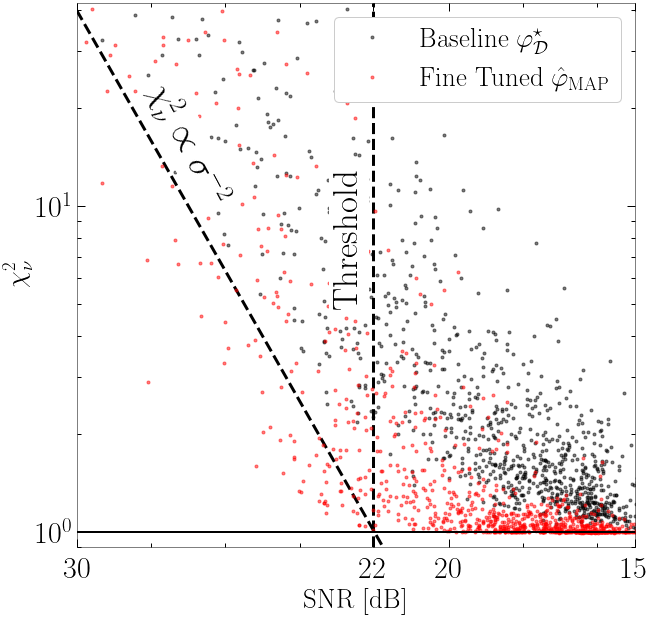
\includegraphics[width=0.8\columnwidth]{figures/chisq_vs_noise_ewc}
        \caption{Goodness of fit as a function of SNR shows a threshold 
        behavior where our method reaches its limit.}
        \label{fig:chi squared vs noise}
\end{figure}

We report the distribution 
of $\chi^2_\nu$ against the noise level in Figure \ref{fig:chi squared vs noise}.
Two behaviors can be identified. For SNR below a certain threshold, the goodness of fit 
of the fine-tuned model is essentially flat around the noise level. 
For SNR above the threshold, 
the goodness of fit follows the trend $\chi^2 \propto \sigma^{-2}$, which 
means the reconstructions have stopped improving on par with the noise level.
We define the threshold at the data point with largest 
SNR value which still 
have statistically significant residuals ($|\chi^2 - \nu| < 296)$. We 
find this threshold value to be $22\, \mathrm{dB}$ based on the test set. 
This is well above the peak SNR value of most HST data 
of known gravitational lenses


\begin{figure*}[ht!]
        \centering
        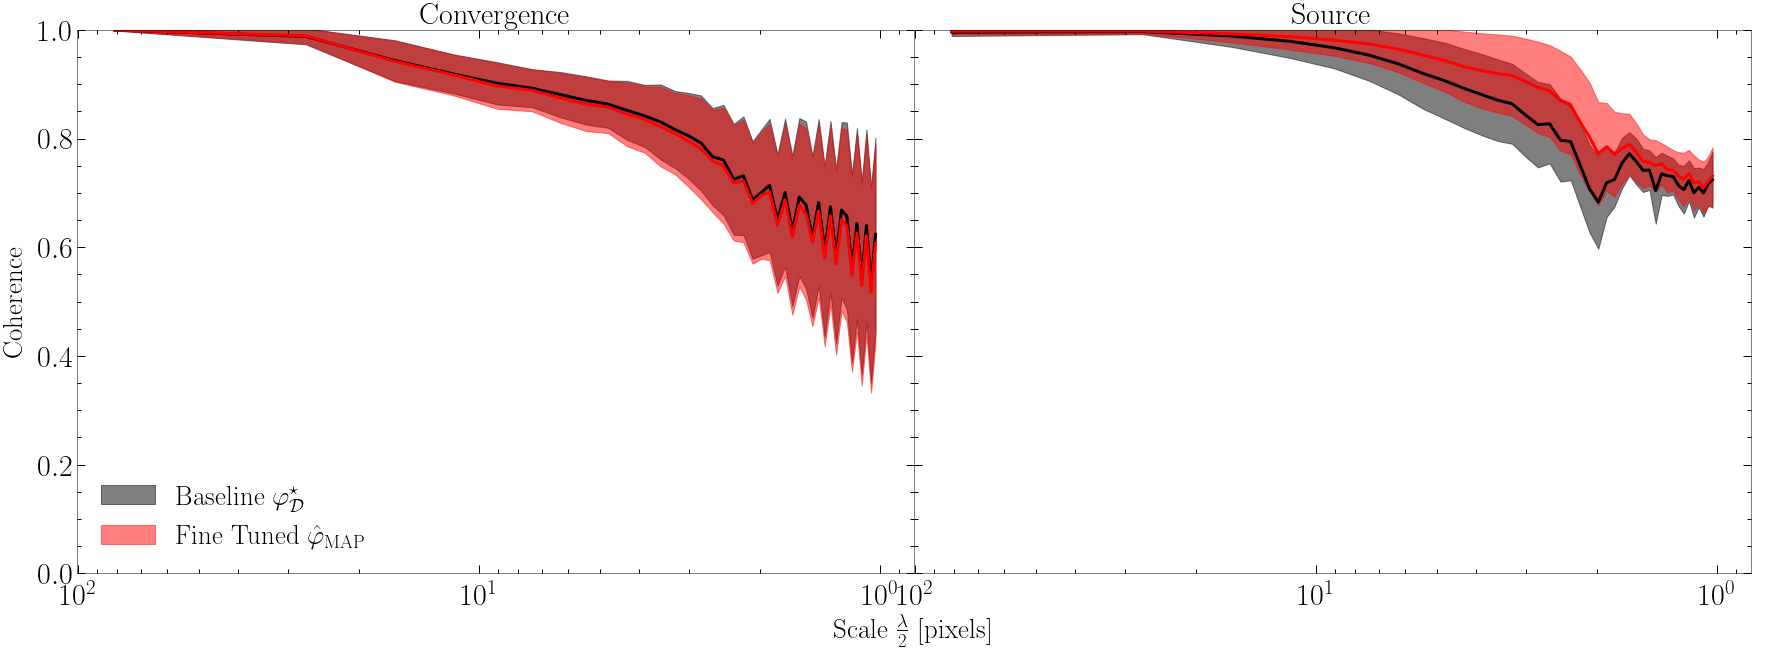
\includegraphics[width=0.8\textwidth]{figures/coherence_spectrum}
        \caption{Statistics of the coherence spectrum on the test set. The solid line is the average 
        coherence. The transparent region is the $68\%$ confidence interval. The fine-tuning 
        procedure yields a noticeable improvement on the coherence of the source at all frequencies.}
        \label{fig:coherence}
\end{figure*}

\subsection{Quality of the Reconstructions}\label{sec:quality of reconstructions}

The loss $\mathcal{L}_\varphi$ by itself is not a strong enough metric to judge the quality 
of the reconstructions. Information about the spatial correlation of pixels 
is lost in that metric. The coherence spectrum encode this information via the cross correlation:
\begin{equation}\label{eq:coherence} 
        \gamma(k) = \frac{P_{12}(k)}{\sqrt{P_{11}(k) P_{22}(k)}}.
\end{equation}
$P_{ij}(k)$ is the cross power spectrum of images $i$ and $j$ at 
the wavenumber $k$. We report the mean value and the $68\%$ confidence interval of those
spectrum in Figure \ref{fig:coherence} 
for the convergence and source maps in the test set. The fine-tuning 
procedure is able to improve significantly the coherence of the background 
source at all scales. The coherence spectrum of the convergence remains unchanged however. 
This is to be expected since there is much fewer constraints on the convergence 
than there are on the background brightness distribution when using only the lensed 
image in the likelihood. 



\section{Conclusion}\label{sec:conclusion}
In this work, we introduced a framework for free-form gravitational 
lensing inference at high SNR. This is an improvement upon traditional modeling. 
Our framework can recover MAP point estimate of both the source and the convergence on pixelated grids 
with high precision and high accuracy, for a wide range of gravitational lensing configurations.

We believe that this framework will enable detailed modelling of present high SNR data and 
upcoming images from facilities like the James Webb Telescope, thereby pushing our understanding of 
dark matter and baryonic matter distribution at the very small scale.


\section{Acknowledgements}
\bibliography{bibliography}

\appendix


\section{Variational Autoencoder (VAE)}\label{ap:VAE}
When working with limited data, data augmentation is crucial to insure that 
the trained model is robust against all sort of perturbations ---
like rotations of an image --- that are not directly included as symmetries in the 
architecture of the model. In that sense, data augmentation is a way to 
induce (or remove) 
a bias via \ref{prior:data} that is not enforced by \ref{prior:architecture}.
In section 
\ref{sec:dataset}, we discuss the different methods for 
augmentations applied to our data. 
In this section, we discuss a generative modelling approach 
to data augmentation that will complement the other ones.

VAEs were originally introduced by \citet{Kingma2013} as a framework to do approximate inference on 
intractable posterior distributions with a latent variable graphical model. 
We aim here to briefly 
cover the most salient concepts related to our work, and refer
the reader to the white paper of \citet{Kingma2019}.

A VAE is decomposed into two parts. On the one hand, an encoder 
$q_\phi$ is a stochastic function which approximate the 
posterior of a latent variable $\mathbf{z}$:
\begin{equation}\label{eq:VAE}
q_{\phi} (\mathbf{z} \mid \mathbf{x}) \approx p_{\theta}(\mathbf{z} \mid \mathbf{x}).
\end{equation} 
On the other hand, the decoder networks with parameters $\theta$ 
is the generative part of the VAE. It learns to decode 
the latent space into meaningful features of the data $\mathbf{x}$. 
In this sense, the generative model goal is to learn a posterior 
of the data $p_{\theta}(\mathbf{x} \mid \mathbf{z})$.
The objective function for this problem 
is the evidence lower bound {($\mathcal{L}_{\phi,\theta}$: ELBO)} 
which aims to satisfy \eqref{eq:VAE}:
\begin{equation}\label{eq:ELBOth}
\mathcal{L}_{\phi,\theta}(\mathbf{x}) =
        \EX_{q_\phi} \big[\log p_{\theta}(\mathbf{x}) \big]
        - D_{\mathrm{KL}}\big(q_\phi(\mathbf{z} \mid \mathbf{x}) \Vert p_\theta (\mathbf{z} \mid \mathbf{x}) \big).
\end{equation} 
To make this problem tractable, we assume the latent 
variable distributions should follow a normal 
distribution with a diagonal covariance matrix: 
\begin{equation}\label{eq:Latent}
        p(\mathbf{z}) \sim \mathcal{N}(0, \bbone)
\end{equation} 
Under the reparameterization trick \citep{Kingma2013}
\begin{equation}\label{eq:Reparametrization}
\begin{aligned}
        \boldsymbol{ \epsilon} &\sim \mathcal{N}(0, \bbone)\\
        (\boldsymbol{\mu}, \log \boldsymbol{\sigma}) &= \mathrm{Encoder}_{\phi}(\mathbf{x})\\
        \mathbf{z} &= \boldsymbol{ \mu} + \boldsymbol{ \sigma} \odot \boldsymbol{ \epsilon},
\end{aligned} 
\end{equation} 
the ELBO 
can then be differentiated w.r.t $\phi$ and $\theta$ since this choice 
yields a tractable ELBO with a functional form 
described by equation (10) of \citet{Kingma2013}:
\begin{equation}\label{eq:ELBO} 
        \mathcal{L}_{\phi,\theta} \simeq 
        \log p_{\theta}(\mathbf{x} \mid \mathbf{z})
        +
        \frac{\beta}{2}\sum_{j=1}^{J} \big( 1 + \log(\boldsymbol{\sigma}_j^{2}) - \boldsymbol{\mu}_j^{2} - \boldsymbol{\sigma}_j^{2}\big).
\end{equation} 
We've introduced the $\beta$ parameters to balance the KL term with the 
reconstruction error as mentionned in section \ref{sec:vae training}.
Once trained, the generative model $\mathrm{Decoder}_\phi (\mathbf{z})$ 
can be used to generate new examples from the latent space $\mathbf{z} \sim \mathcal{N}(0, \bbone)$.



\section{Autoencoder}\label{ap:AE}



\section{Elastic Weight Consolidation}\label{ap:ewc}
Suppose we are given a training set $\mathcal{D}$ and a test task $\mathcal{T}$. The 
posterior of the RIM parameters $\mathcal{\varphi}$ can be rewritten using the Bayes rule as
\begin{equation}
        p(\varphi \mid \mathcal{D},\, \mathcal{T}) = 
        \frac{p(\mathcal{T} \mid \mathcal{D},\, \varphi) p(\varphi \mid \mathcal{D})}
        {p(\mathcal{T} \mid \mathcal{D})}.
\end{equation} 
We suppose that $\varphi$ encode 
information about $\mathcal{D}$, while $\mathcal{T}$ was unseen by $\varphi$. 
It follows that 
$\mathcal{T}$ and $\mathcal{D}$ are conditionally independent when given $\varphi$. 
We do not make the stronger assumption that $\mathcal{D}$ and $\mathcal{T}$ 
are completely independent. In fact, such an assumption 
would contradict the premiss of our work that building a 
dataset $\mathcal{D}$ can inform a machine $G_\varphi$ about
task $\mathcal{T}$ --- or that, more broadly, $\mathcal{D}$ 
contains information about $\mathcal{T}$.

We rewrite the marginal $p(\mathcal{T} \mid \mathcal{D})$ using the Bayes rule
in order to extract the sampling distribution used to compute 
the Fisher diagonal elements $p(\mathcal{D} \mid \mathcal{T})$ s.t.
\begin{equation}
        p(\varphi \mid \mathcal{D},\, \mathcal{T}) = 
\frac{p(\mathcal{T} \mid \varphi) p(\varphi \mid \mathcal{D})}
        {p(\mathcal{D} \mid \mathcal{T})}
        \frac{p(\mathcal{T})}{p(\mathcal{D})}.
\end{equation} 
The log-likelihood $\log p(\mathcal{T} \mid \varphi)$ is equivalent to 
the negative of the loss function for the particular task at hand.
In this work, we assign a uniform probability density to $p(\mathcal{T})$ and $p(\mathcal{D})$ 
in order to ignore them.

We now turn to the prior $p(\varphi \mid \mathcal{D})$, which 
appears as a conditional relative to 
the training dataset. 
We use the Laplace approximation around the maxima $\varphi^{\star}_{\mathcal{D}}$ 
to evaluate the prior,
where $\varphi^{\star}_{\mathcal{D}}$ 
are the trained parameters (learned with dataset $\mathcal{D}$) 
that minimize the training cost. The Taylor expansion 
of the prior around this maxima yields
\begin{equation}\label{app:prior}
        \log p(\varphi \mid \mathcal{D}) \approx \log p(\varphi^{\star}_{\mathcal{D}} \mid \mathcal{D}) 
        + \frac{1}{2} (\varphi - \varphi^{\star}_{\mathcal{D}})^{T} 
        \underbrace{
        \bigg(
                \frac{\partial^2 \log p(\varphi \mid \mathcal{D})}{\partial^2 \varphi}\bigg|_{\varphi^{\star}_{\mathcal{D}}}
        \bigg)
}_{\displaystyle \mathbf{H}(\varphi^{\star}_{\mathcal{D}})}
        (\varphi - \varphi^{\star}_{\mathcal{D}}).
\end{equation} 
Since $\varphi^{\star}_{\mathcal{D}}$ is an extrema of the prior, the linear term vanishes. 
The empirical estimate of the negative hessian matrix is the observed Fisher information 
matrix which can be written as
\begin{equation}\label{app:fisher}
        \mathcal{I}(\varphi^{\star}_{\mathcal{D}}) = 
        -\EX_{\mathcal{D} \mid \mathcal{T}} [\mathbf{H}(\varphi^{\star}_{\mathcal{D}})] = 
        \EX_{\mathcal{D}\mid \mathcal{T}}
        \Bigg[
                \Bigg(
                \bigg( 
                        \frac{\partial \log p(\varphi \mid \mathcal{D})}{\partial \varphi}
                \bigg) 
                \bigg( 
                        \frac{\partial \log p(\varphi \mid \mathcal{D})}{\partial \varphi}
                \bigg)^{T}
        \Bigg)
\Bigg|_{\varphi^{\star}_{\mathcal{D}}}\Bigg].
\end{equation} 
The expectation is taken over the sample space $p(\mathcal{D} \mid \mathcal{T})$ since 
the network parameters are held fixed during sampling.
In order to compute the Fisher score, 
we apply once more the Bayes rule to extract a loss function:
\begin{equation} 
        \log p(\varphi \mid \mathcal{D}) = \log p(\mathcal{D}\mid \varphi) 
        + \log p(\varphi) - \log p(\mathcal{D}).
\end{equation} 
$p(\mathcal{D} \mid \varphi)$ is the negative of a loss function. 
We use a rescaled version of \eqref{eq:Loss}:
\begin{equation}\label{eq:LossFisher} 
        \log p((\mathbf{x},\mathbf{y}) = \mathcal{D} \mid \varphi) = -TM \mathcal{L}_{\varphi}(\mathbf{x},\mathbf{y}),
\end{equation} 
where $M$ is the total number of pixels in $\mathbf{x}$ and $T$ is the 
total number of steps for the recurrent inference machine.
The rescaling removes the artificial temperature added to the 
loss during training. 
The derivative of $\log p(\varphi)$ remains constant when taking 
the expectation of \eqref{app:fisher}. If needed, 
it can be modeled with a traditional $\ell_2$ loss. But, we find that 
this term can safely be ignored.

Since the full Fisher matrix is intractable for a neural network, we approximate the 
quadratic term of the prior with the diagonal of the Fisher matrix following \citet{Kirkpatrick2016}. 
For an optimisation problem, the first term of \eqref{app:prior} is constant. Thus,
the posterior becomes proportional to
\begin{equation}
        \log p(\varphi \mid \mathcal{D}, \mathcal{T}) \propto 
        \log p(\mathcal{T} \mid \varphi ) - 
         \frac{\lambda}{2} 
        \sum_{j}[\mathcal{I}(\varphi^{\star}_{\mathcal{D}})]_{jj}(\varphi_j - \varphi^{\star}_{\mathcal{D},j})^2.
\end{equation} 
The Lagrange multiplier $\lambda$ is introduced to weight the importance of the regularisation 
during fine-tuning.

\begin{figure*}[ht!]
        \centering
        \begin{tikzpicture}
                \node at (0, 0) {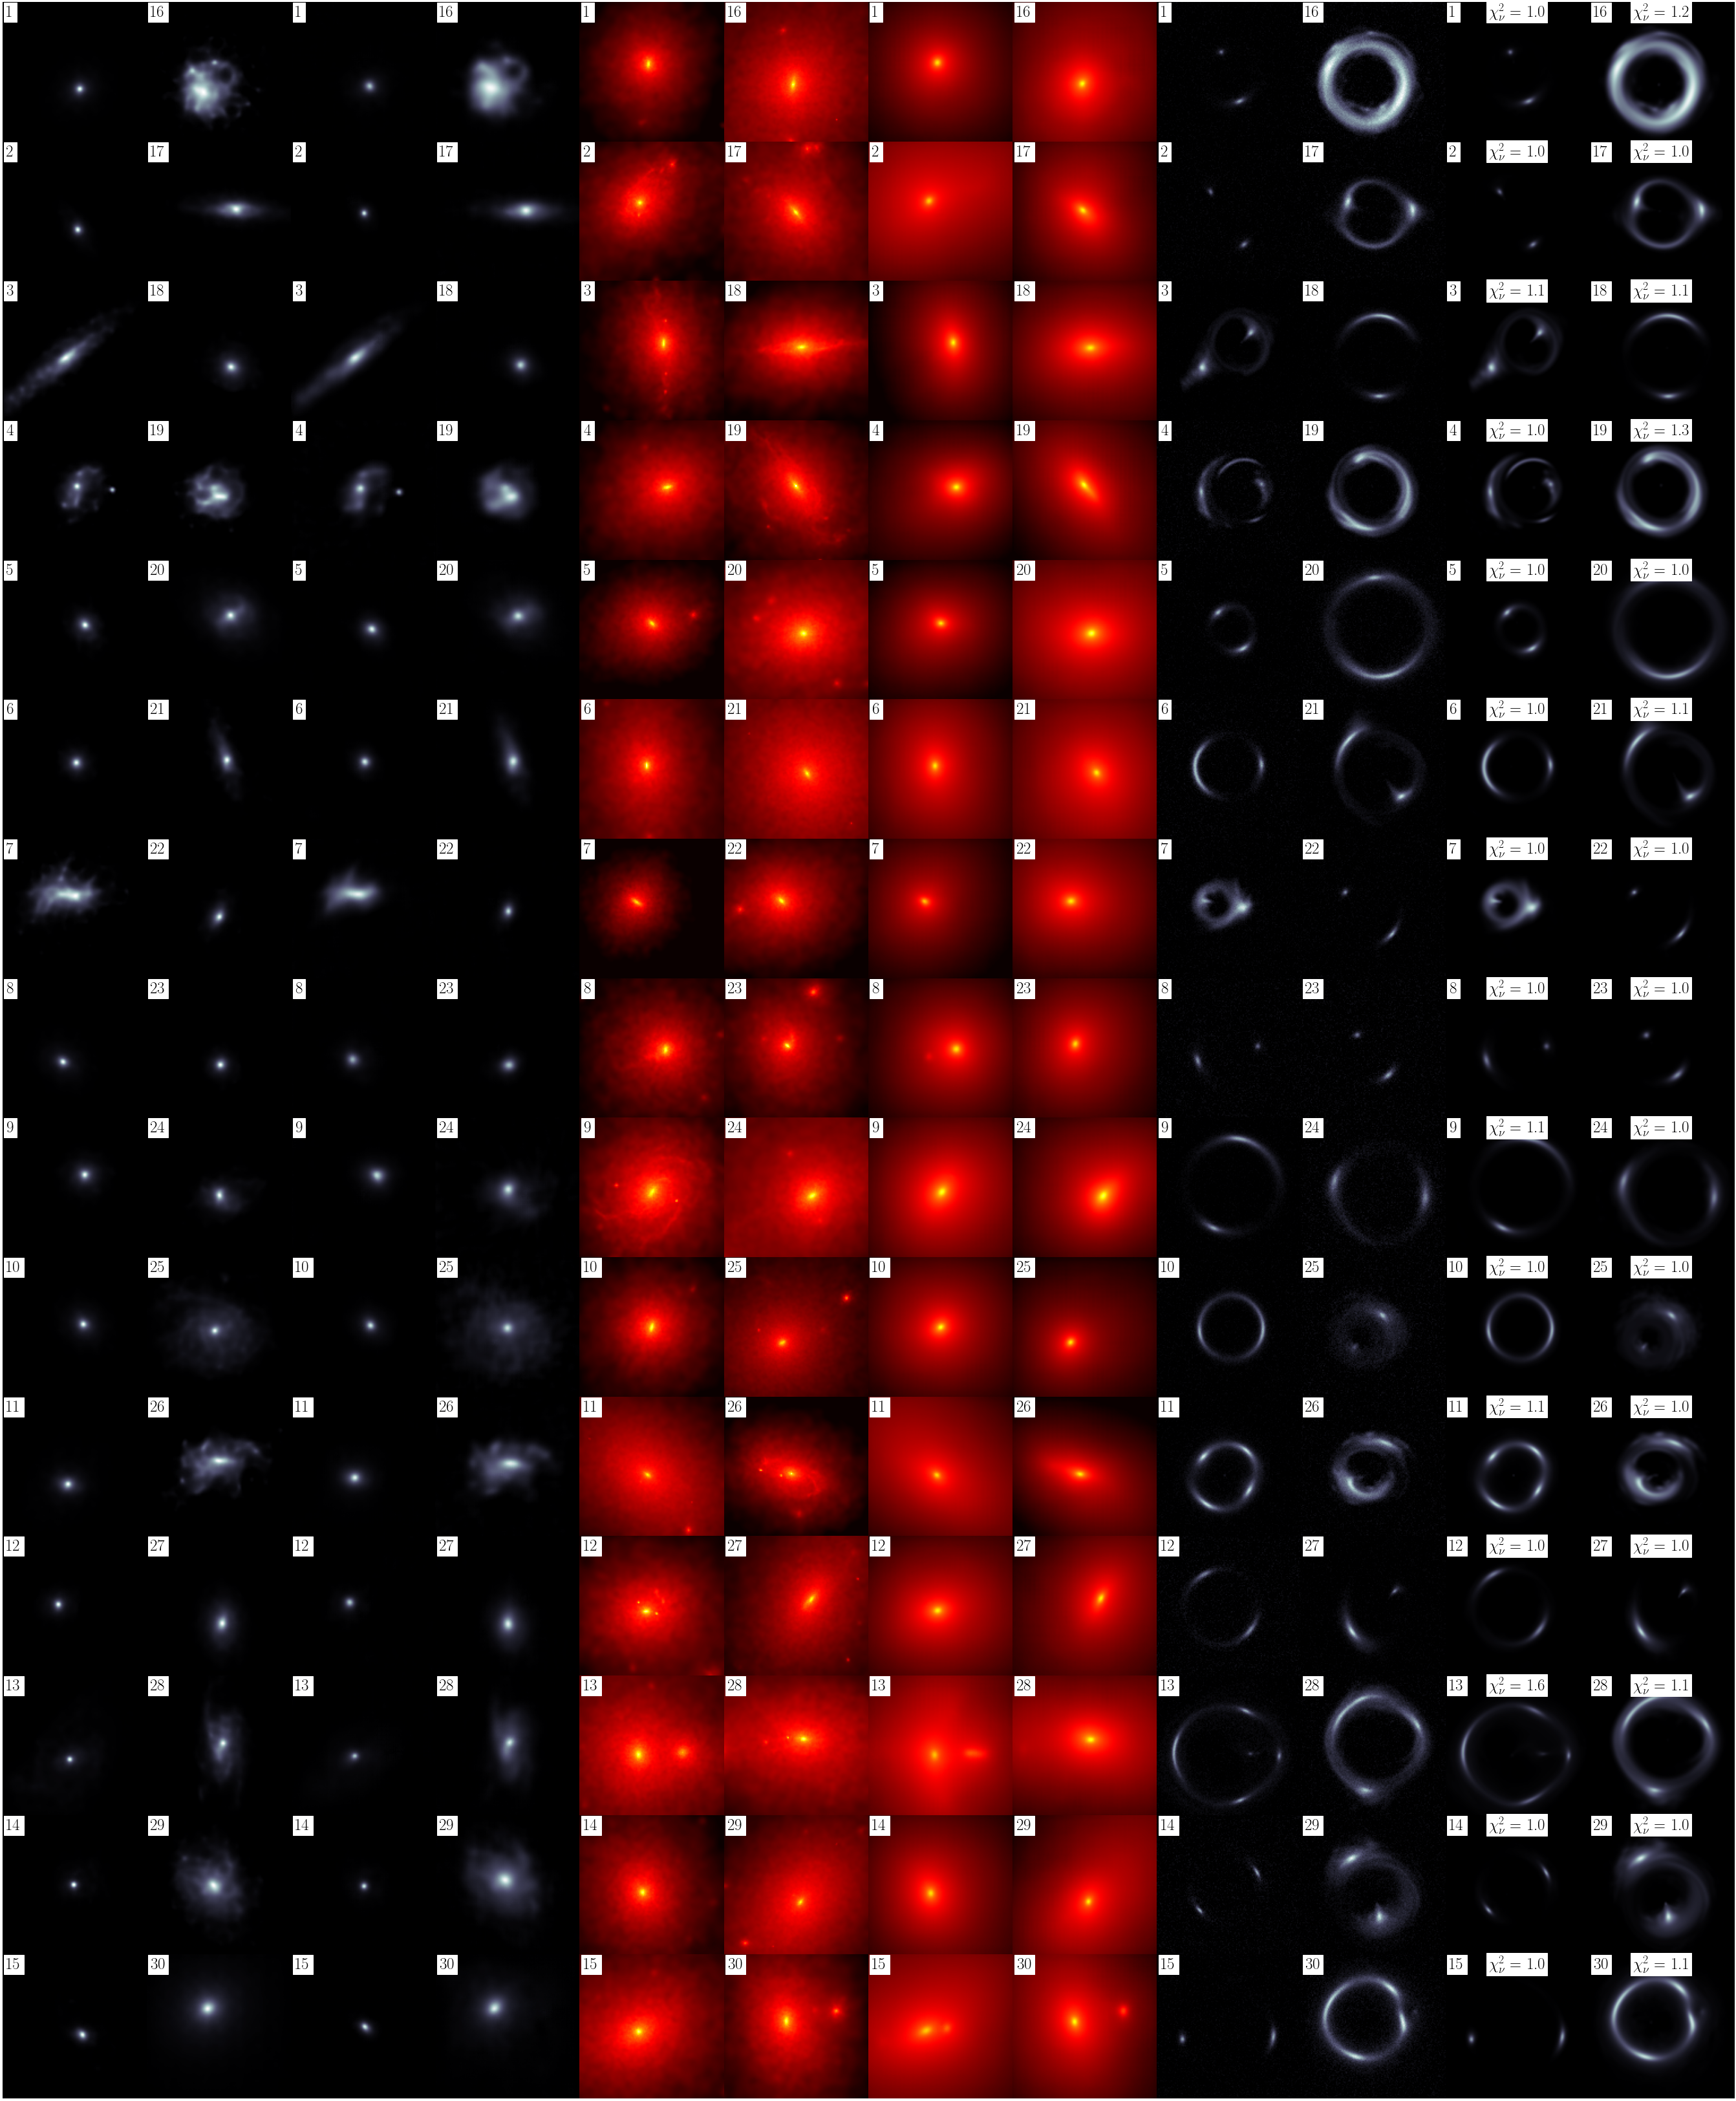
\includegraphics[width=\linewidth]{figures/test_set_rim_pred_no_cherry_pick}};
                \node at (-7.5, 11.2) {COSMOS};
                \node at (-4.5, 11.2) {RIM+FT};
                \node at (-6, 11.7) {Sources};
                \node at (-1.5, 11.2) {Illustris TNG};
                \node at (1.5, 11.2) {RIM+FT};
                \node at (0, 11.7) {Convergence};
                \node at (4.5, 11.2) {Observation};
                \node at (7.5, 11.2) {RIM+FT};
        \end{tikzpicture}
        \caption{
                30 reconstructions taken at random from the test set of 3000 examples simulated from COSMOS 
                and IllustrisTNG data at high SNR.
                The colorscale are the same as in Figure \ref{fig:main result}.}
        \label{fig:random sample}
\end{figure*}


\begin{figure*}[ht!]
        \centering
        \tikzset{font={\fontsize{8pt}{12}\selectfont}}
        \begin{tikzpicture}
                \draw[-latex] (-8, 3.5) -- (-8, -3.5) node[midway, above, rotate=90] {Increasing SNR};
                \node at (0, 0) {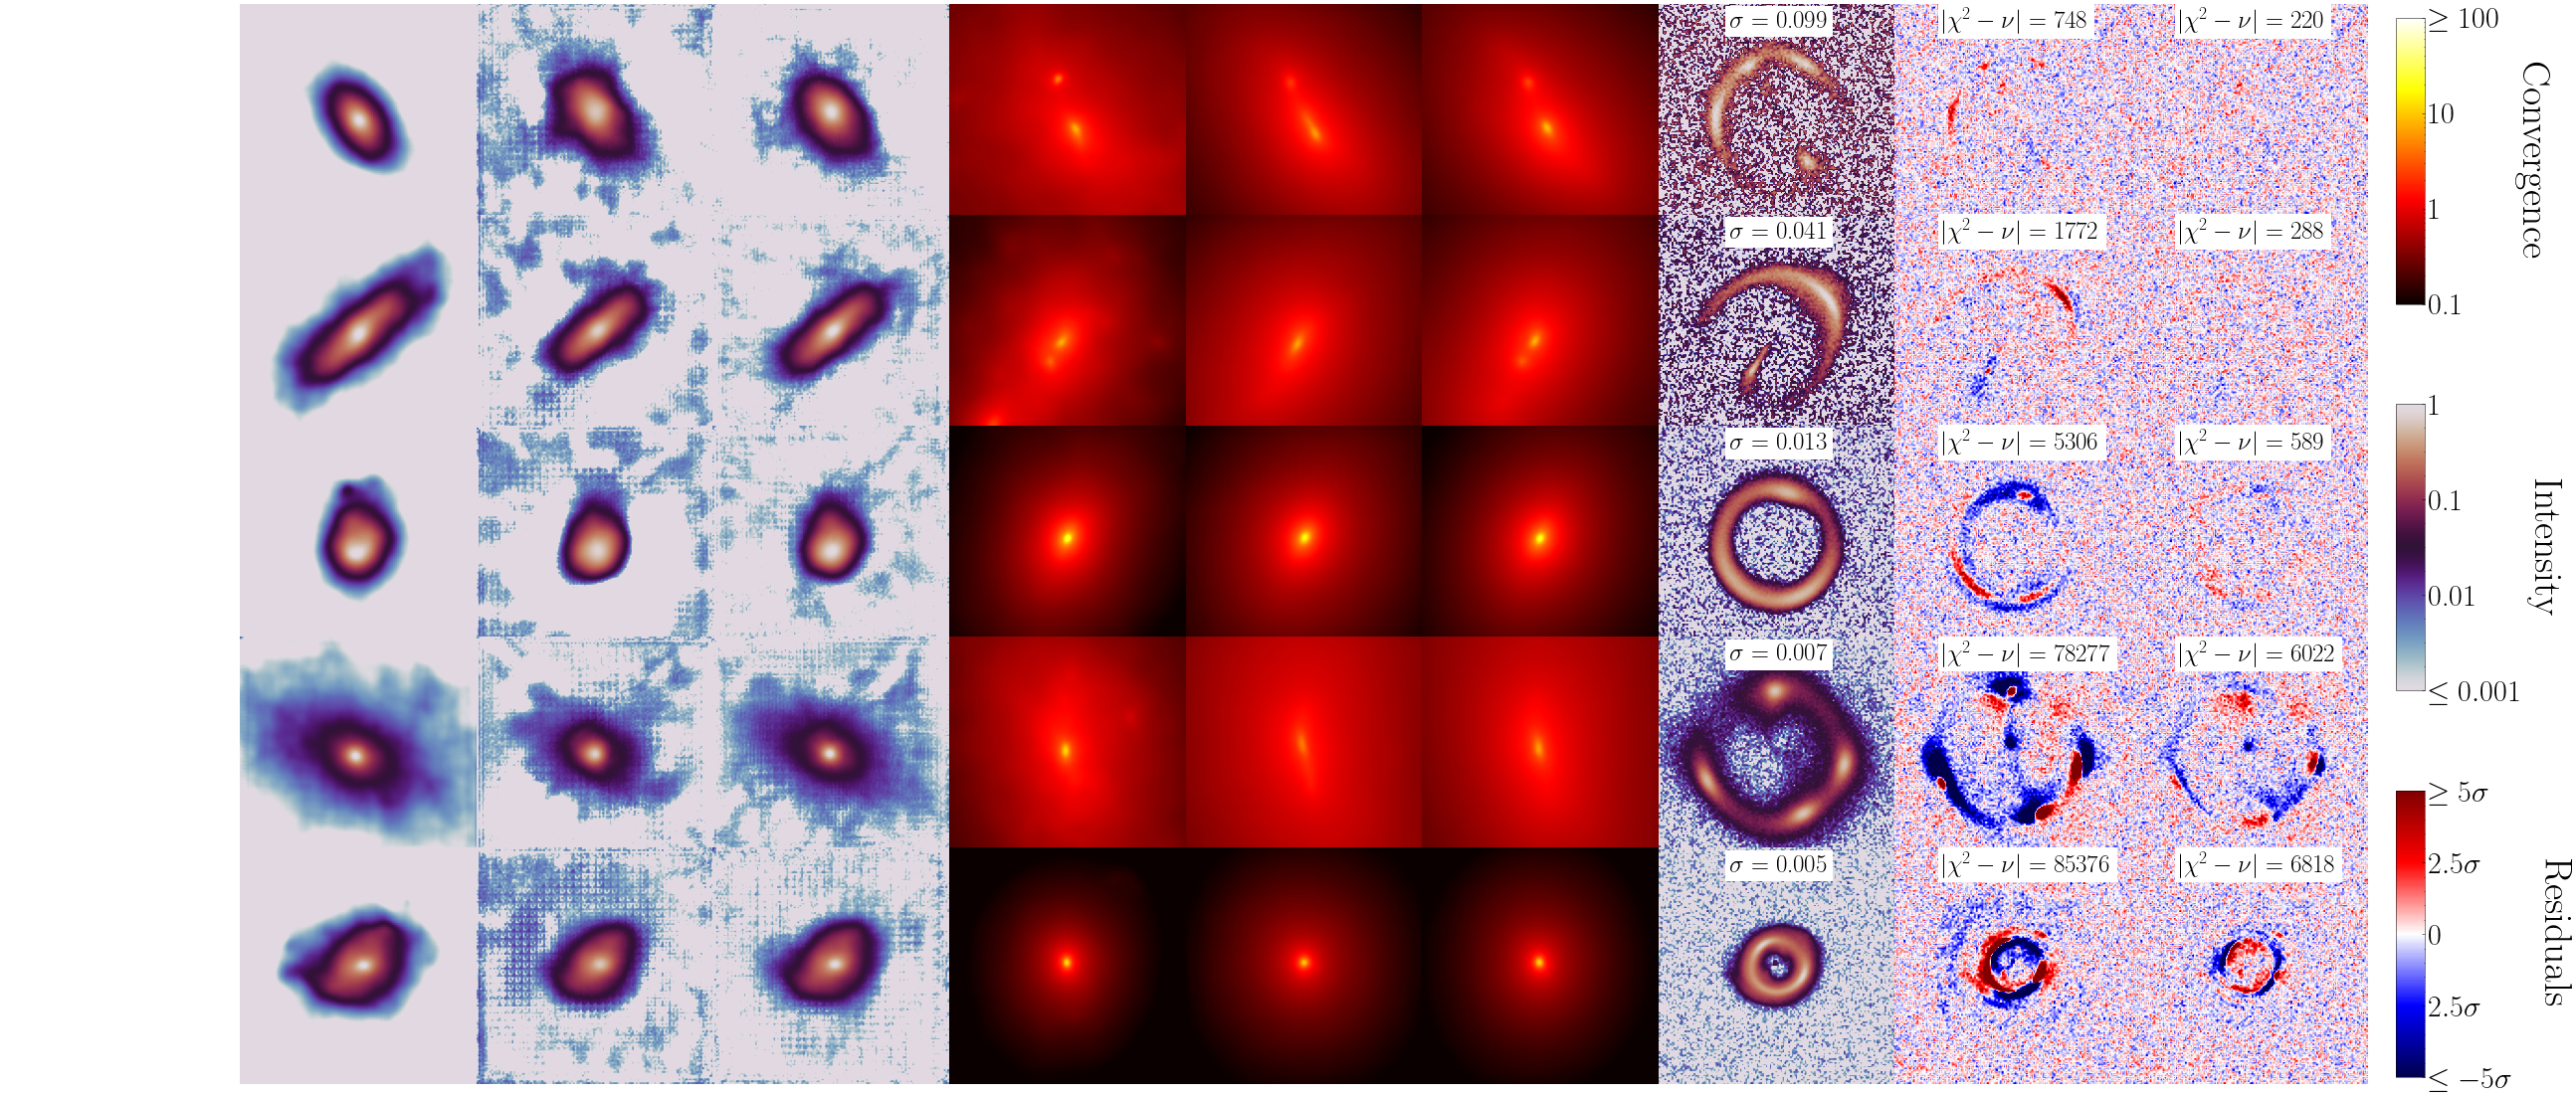
\includegraphics[width=\linewidth]{figures/rim_map_on_vae_cherry_picks}};
                \node at (-6.5, 4.5) {Source};
                \node at (-4, 4.5) {Reconstruction};
                \node at (-6.5, 4.1) {VAE};
                \node at (-4.9, 4.1) {RIM};
                \node at (-3.2, 4.07) {RIM+FT};
                \node at (-1.5, 4.5) {Convergence};
                \node at (1, 4.5) {Reconstruction};
                \node at (-1.5, 4.1) {VAE};
                \node at (0.1, 4.1) {RIM};
                \node at (1.7, 4.07) {RIM+FT};
                \node at (3.5, 4.1) {Observation};
                \node at (5.8, 4.5) {Residuals};
                \node at (5, 4.1) {RIM};
                \node at (6.7, 4.07) {RIM+FT};
        \end{tikzpicture}
        \caption{
        Comparison between baseline and MAP estimate of the weights of the RIM for VAE samples. 
        The examples chosen are representative 
        of the larger sample. From top to bottom, we increase SNR. The first 2 
        rows have noise level reconstruction, while the last 3 row show significant improvement 
        over the baseline. The intensity color scale is chosen to show the reconstruction
down to the third decimal place, where the baseline prediction breaks down.}
\end{figure*}


\end{document}

